\documentclass[12pt]{article} 

% Adjust margining to narrow
\usepackage{geometry}
\geometry{a4paper, total={170mm,257mm}, left=20mm, top=20mm}

% Mathematics font
\usepackage{amsfonts}
\usepackage{amsmath}

% Graphics import
\usepackage{graphicx}
\usepackage{subcaption}
\graphicspath{{C:/Users/user/Desktop/KUL - Mstat/Big Data Platforms and Technologies/report/graph}}

% Advanced table
\usepackage{tabularx}
\usepackage{makecell}

% No indentation
\setlength\parindent{0pt}

% ------------------------------------------------------------------------
% Assignment content
\begin{document}
\begin{titlepage}
	\begin{center}
	\vspace*{1cm}
    
\includegraphics[width=0.4\textwidth]{KUL}\\
	\vspace{2.5cm}
    {\Large Report for Advanced Analytics in Business}
            
    \vspace{1.5cm}

    {\large Ana Maria Giraldo Vargas, r0822450}\\
    \vspace{0.5cm}
    {\large David Badajkov, r0604517}\\
    \vspace{0.5cm}
    {\large Marcela 	Lopez Viveros, r0773141}\\
	\vspace{0.5cm}
	{\large Sonia Rocio 	Socadagui Casas, r0823960}\\
	\vspace{0.5cm}
    {\large Wai Chun Cheung, r0817438}
    \vspace{1.5cm}


       \today
   \end{center}
\end{titlepage}

% ------------------------------------------------------------------------
\newpage
\tableofcontents
\newpage

\section*{Assignment 1}
\addcontentsline{toc}{section}{Assignment 1}


\subsection*{Feature engineering}
\addcontentsline{toc}{subsection}{Feature engineering}

The (training) dataset for Assignment 1 consists of 55,463 observations and 78 features. The number of features. It is easy to observe that there are a lot of missing values and categorical or date features in the dataset. In this section, we would discuss the strategies used in handling such problems. 

\subsubsection*{Missing values}
\addcontentsline{toc}{subsubsection}{Missing values}

As shown in figure 1, there are 55 feature which contain missing values, and 24 out of them contain more than 80\% of missing values. For those features with a high proportion of missing values (more than 50\%), missing values are treated as an extra category. By treating missing values as an extra category called \textit{unknown}, the information of the non-missing entries of those features can be retained and learnt by the model, whereas removal of those features may lead to a loss in information or pattern. For those features with a lower proportion of missing values (less than 50\%), some imputation techniques can be applied to estimate their possible values. Another kind of missing values visualization using \texttt{missingno} is presented in figure 2. 

\begin{figure}[h]
\centering
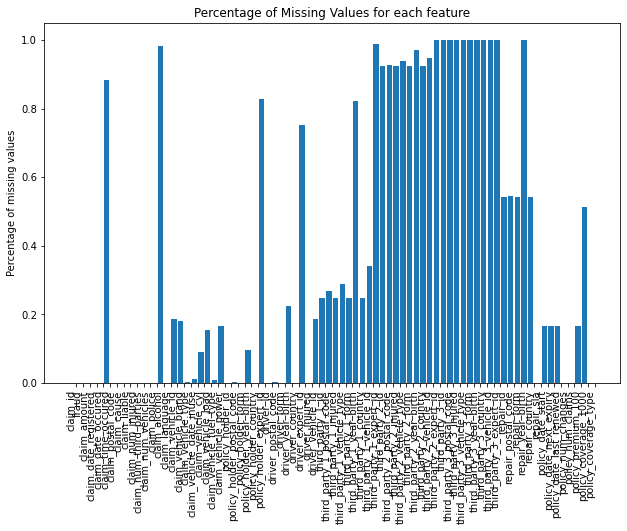
\includegraphics[width=1\linewidth]{missing_value_plt1}
\caption{Proportions of missing values for each feature}
\end{figure}

\begin{figure}[h]
\centering
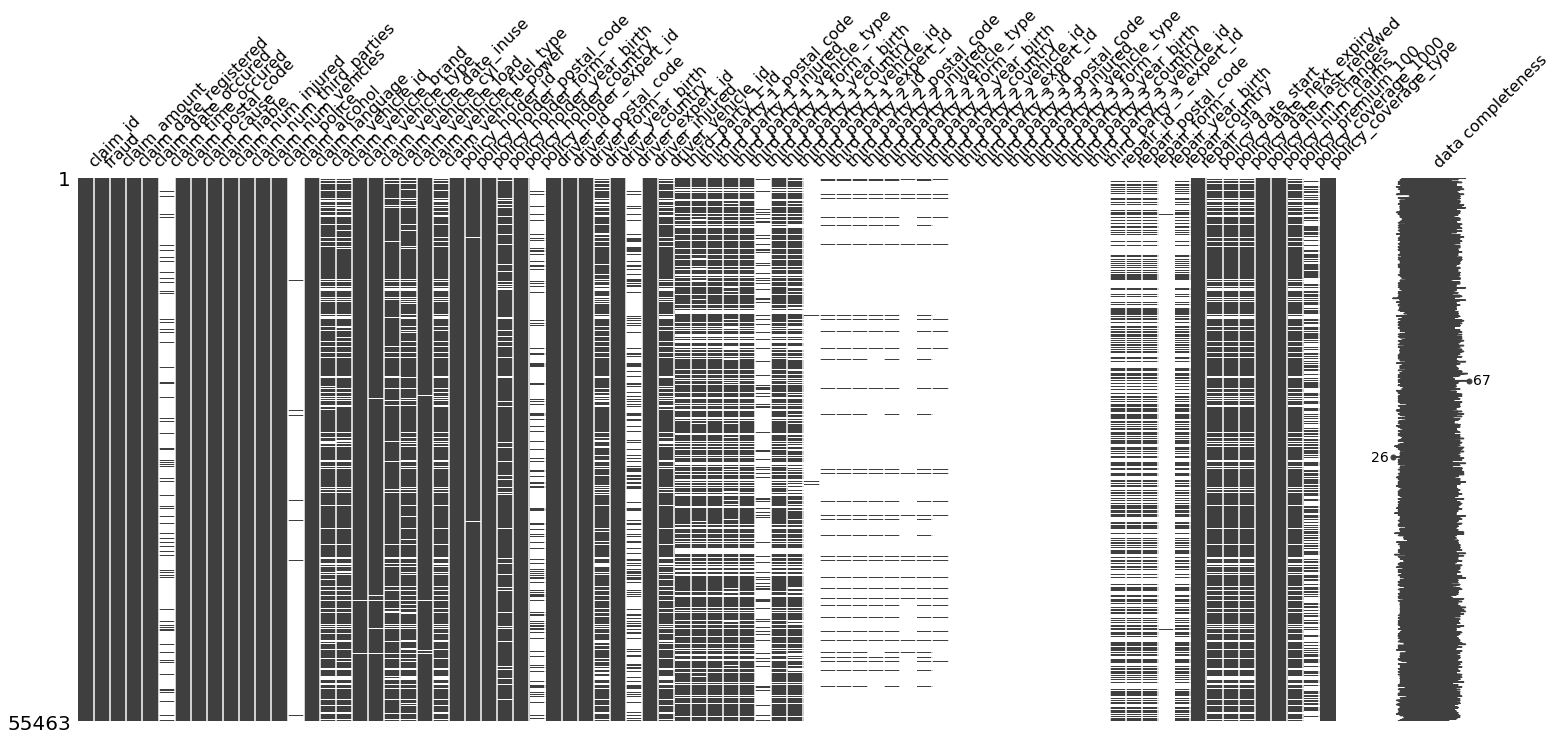
\includegraphics[width=1\linewidth]{missing_value_plt2}
\caption{Visualization of missing values with \texttt{missingno} python library}
\end{figure}

\subsubsection*{Date features}
\addcontentsline{toc}{subsubsection}{Date features}

Some features are available in form of date. In the dataset, the following features are in terms of date: \texttt{claim\_date\_registered}, \texttt{claim\_date\_occured}, \texttt{claim\_vehicle\_date\_inuse}, \texttt{policy\_date\_start}, \texttt{policy\_date\_next\_expiry} and \texttt{policy\_date\_last\_renewed}. However, date itself is not suitable to serve as an input for some machine learning models. Hence, as summarized in table 1, we construct another set of features which are more interpretable and meaningful based on these date features.\\

Apart from the aforementioned features, features related to birth year are also considered as date features. They are \texttt{policy\_holder\_year\_birth}, \texttt{driver\_year\_birth}, \texttt{third\_party\_1\_year\_birth}, \texttt{third\_party\_2\_year\_birth}, \texttt{third\_party\_3\_year\_birth} and \texttt{repair\_year\_birth} in the dataset. By subtracting them from the year of \texttt{claim\_date\_occured}, we obtain age-related features.

\begin{table}[h]
	\begin{tabular}{|l|p{11.5cm}|}
	\hline
	Constructed features & Descriptions\\
	\hline
	\texttt{days\_before\_registered} & The number of days between \texttt{claim\_date\_registered} and \texttt{claim\_date\_occured}.\\
	\hline
	\texttt{days\_before\_occured} & The number of days between \texttt{claim\_date\_occured} and \texttt{claim\_vehicle\_date\_inuse}.\\
	\hline
	\texttt{policy\_length} & The number of days between \texttt{policy\_date\_last\_renewed} and \texttt{policy\_date\_start}.\\
	\hline
	\texttt{policy\_claim\_length} & The number of days between \texttt{policy\_date\_next\_expiry} and \texttt{claim\_date\_occured}.\\
	\hline
	various age-related features & The number of years between the year of \texttt{claim\_date\_occured} and birth year.\\	
	\hline
	\end{tabular}
	\caption{Featurization of date features}
\end{table}

\vspace{-1cm}
\subsubsection*{Data quality issue}
\addcontentsline{toc}{subsubsection}{Data quality issue}

During data cleaning process, we discovered some problems with regards to data quality. For example, the instance with claim id 62780 has an invalid value for the year of \texttt{claim\_vehicle\_date\_\\inuse}. Such observations may be due to input error in manual data entering process. In this case, we may manually correct the year from 2705 to 2005. However, they can be hard and time-consuming to observe in general. A separate data validation process should be carried out before data analysis.

\begin{figure}[h]
\centering
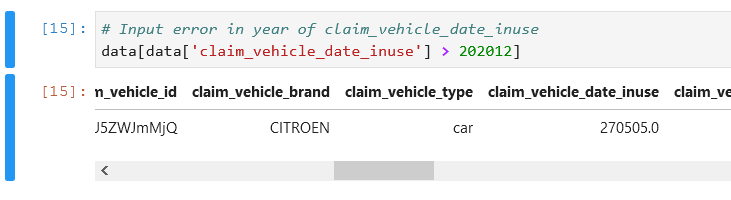
\includegraphics[width=1\linewidth]{data_quality_issue}
\caption{Invalid value of \texttt{claim\_vehicle\_date\_inuse} with claim id 62780}
\end{figure}


\vspace{-1cm}
\subsubsection*{Data binning}
\addcontentsline{toc}{subsubsection}{Data binning}

Binning continuous features can help incorporating missing values and extreme values in a more natural way as they can be reformulated as categorical features. It is useful for those continuous features with a high proportion of missing values or highly right-skewed. For age-related features, they are binned by age groups with equal intervals. In our case, age-related features are encoded into the following categories: $(0, 20], (20, 40], (40, 60], (60, 80], (80, \infty]$ and \textit{unknown}. Equal intervals of 20 years seem to be a reasonable choice by looking at their histograms. For driver age and policy holder age, the density looks like bimodal with a local minima around 40 years. Moreover, extreme ages, which are below 20 and above 80, can be handled properly under such binning. 

\begin{figure}[h]
\centering
\begin{subfigure}{.5\textwidth}
  \centering
  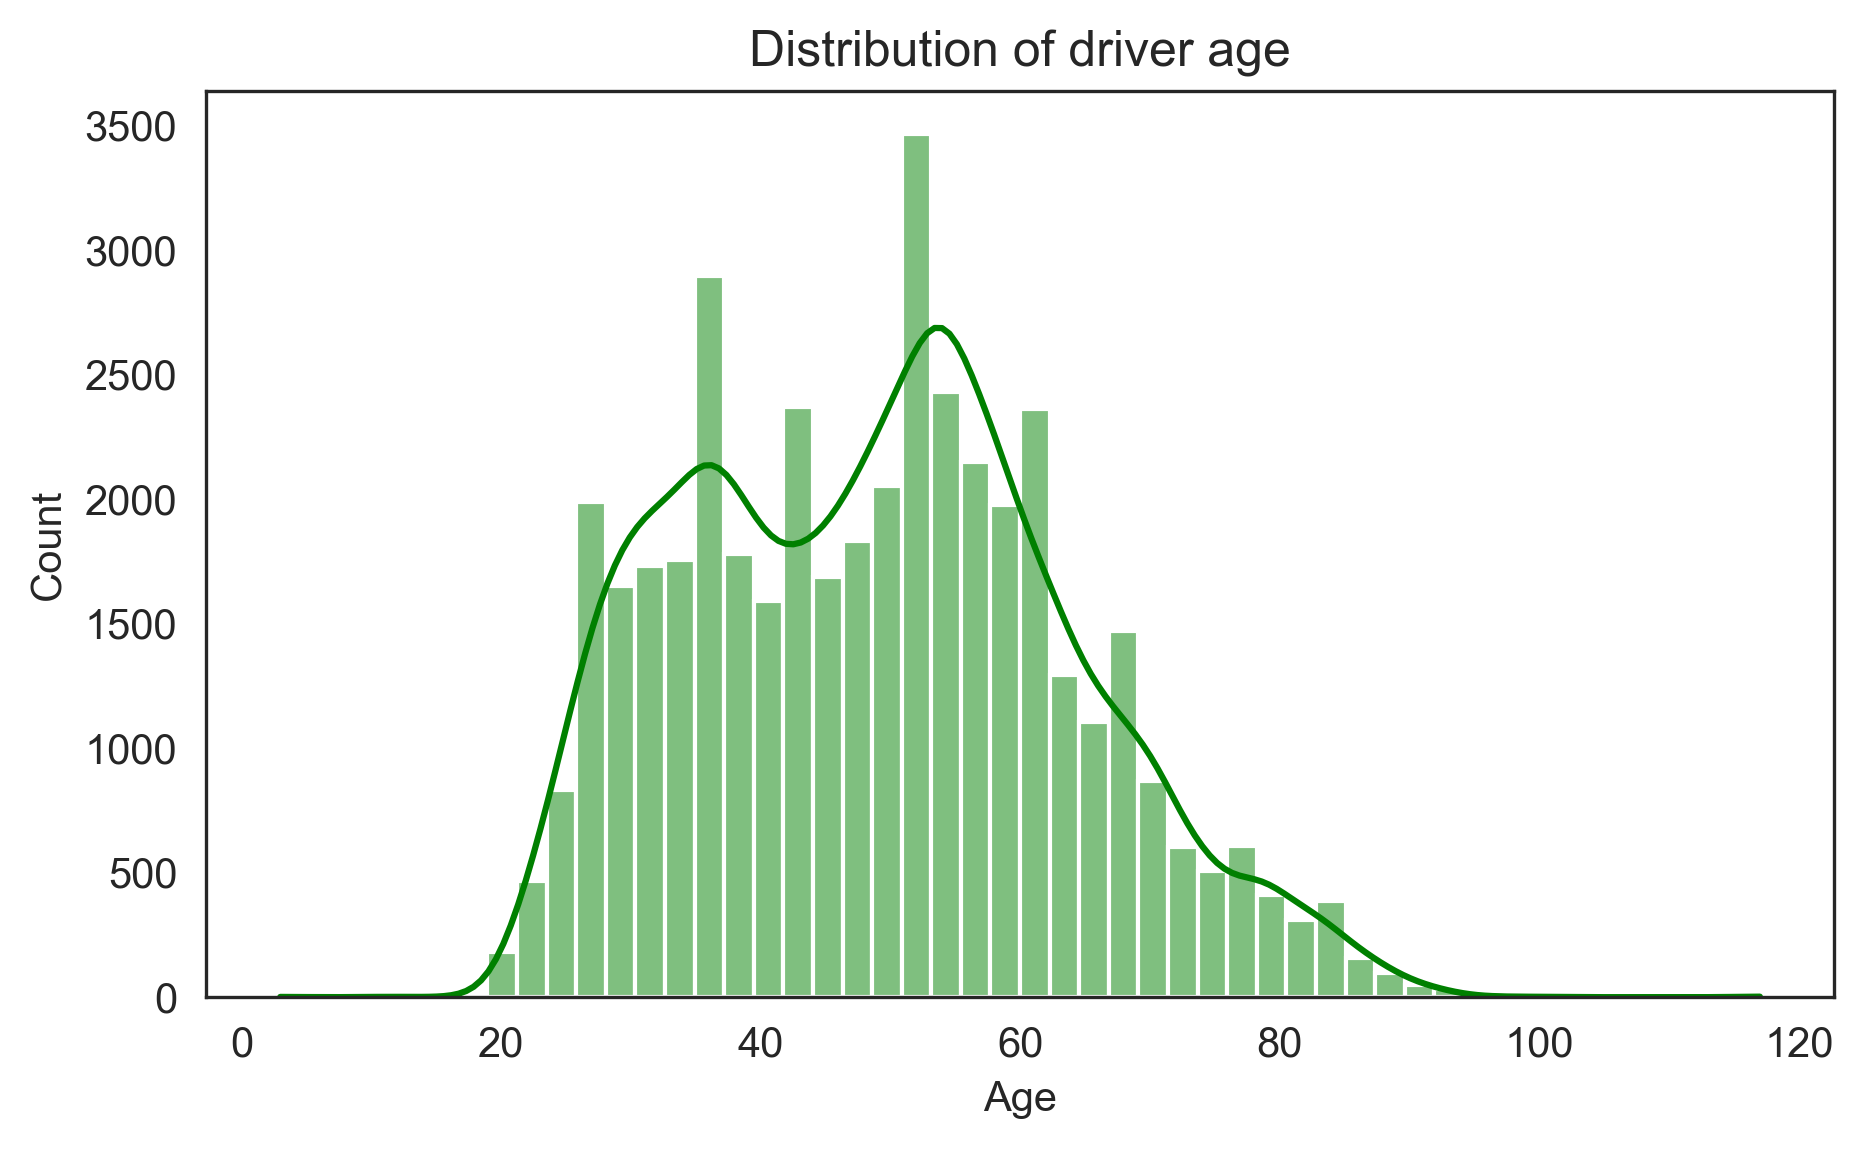
\includegraphics[width=1\linewidth]{dist_driver_age}
  \label{fig:sub1}
\end{subfigure}%
\begin{subfigure}{.5\textwidth}
  \centering
  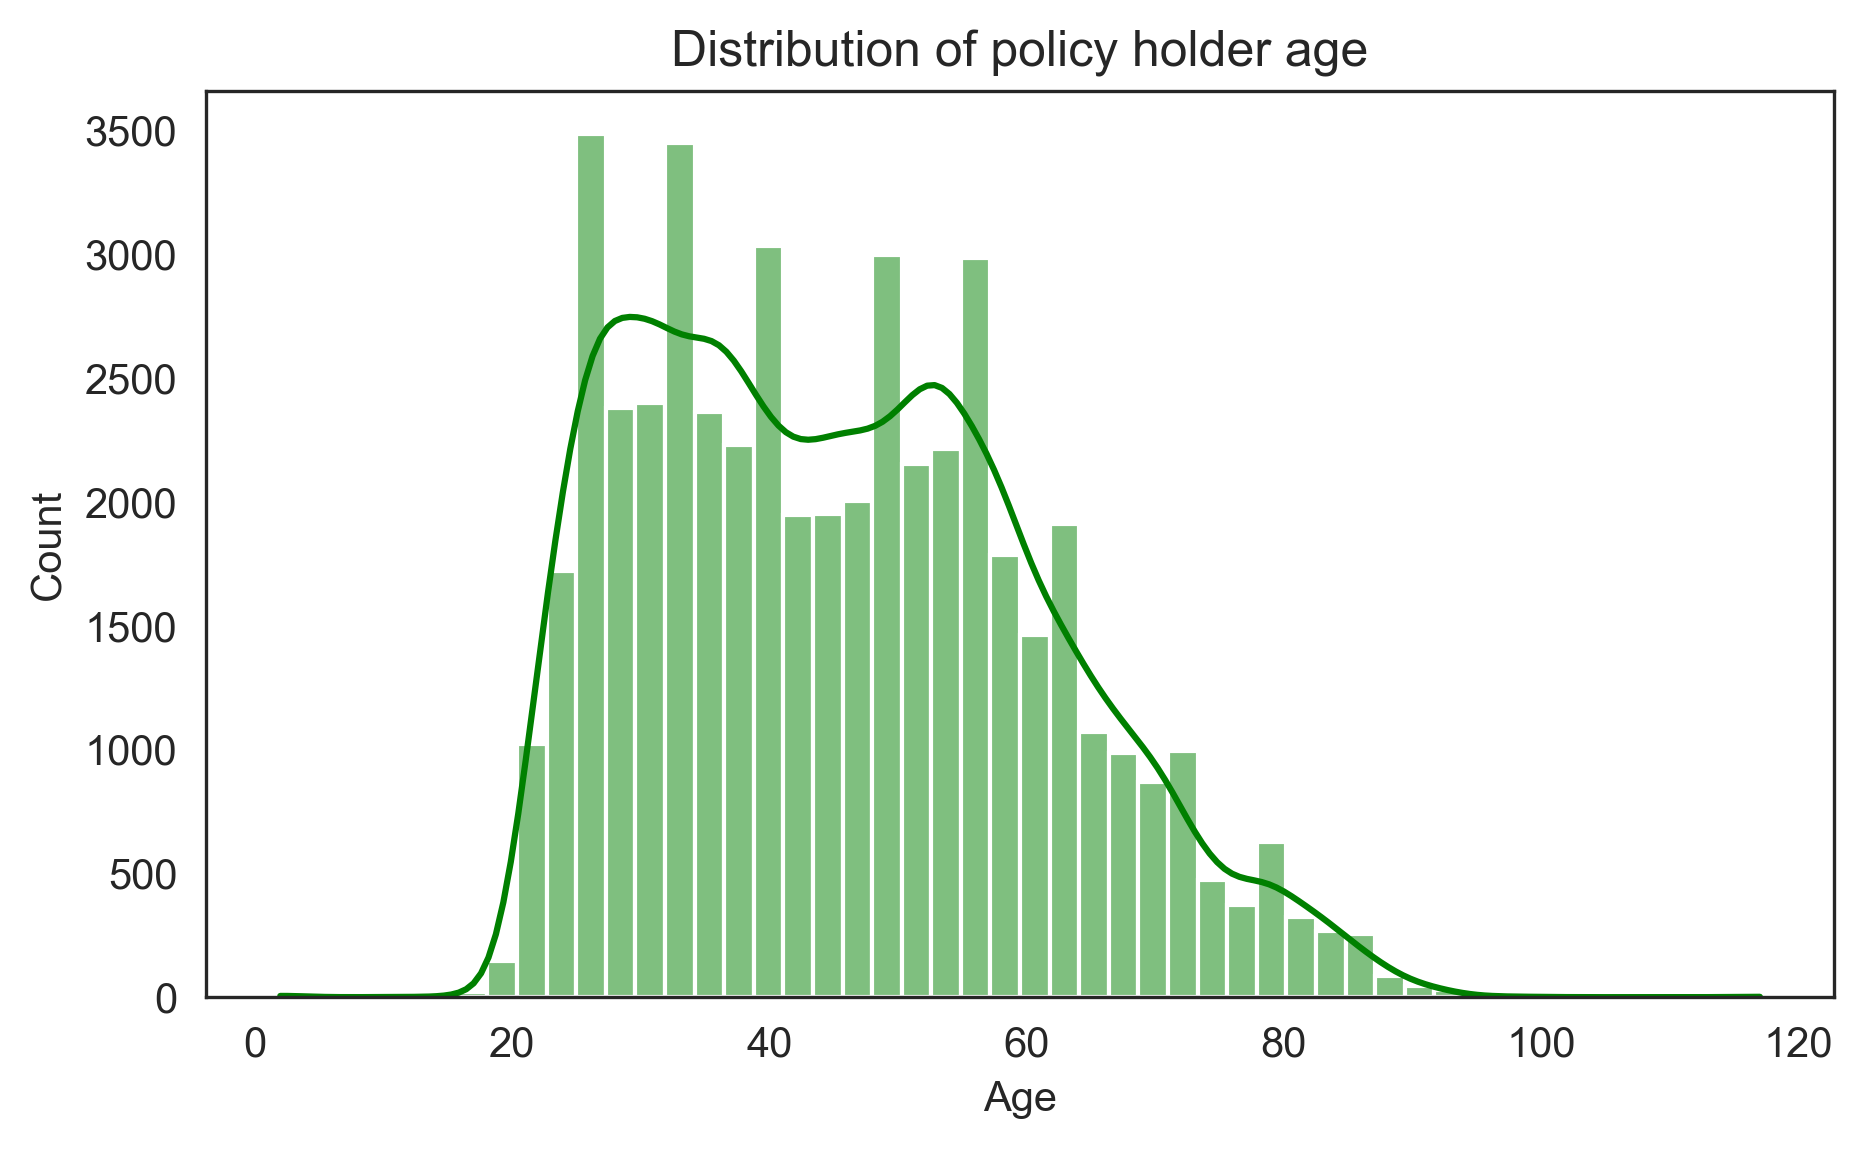
\includegraphics[width=1\linewidth]{dist_policy_holder_age}
  \label{fig:sub2}
\end{subfigure}
\vspace{-1cm}
\begin{subfigure}{.5\textwidth}
  \centering
  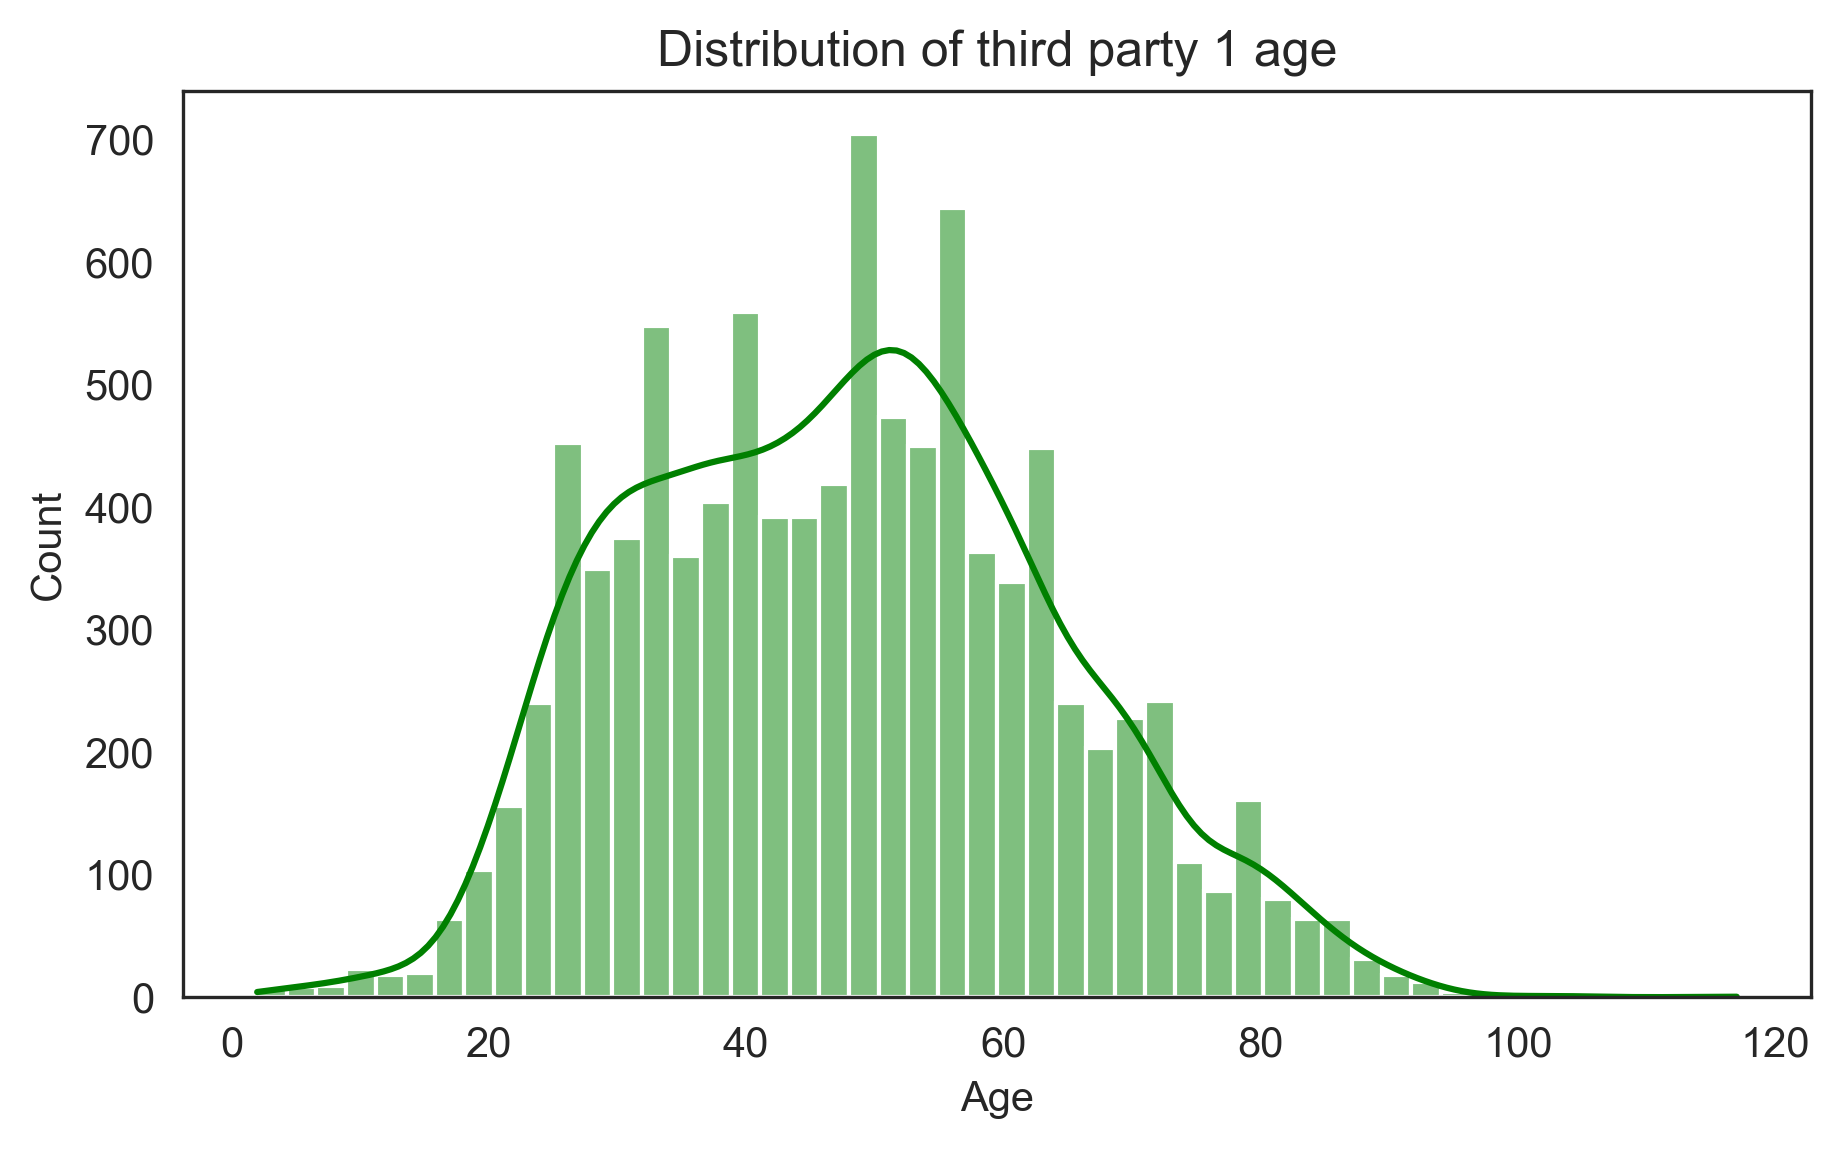
\includegraphics[width=1\linewidth]{dist_third_party_1_age}
  \label{fig:sub3}
\end{subfigure}%
\begin{subfigure}{.5\textwidth}
  \centering
  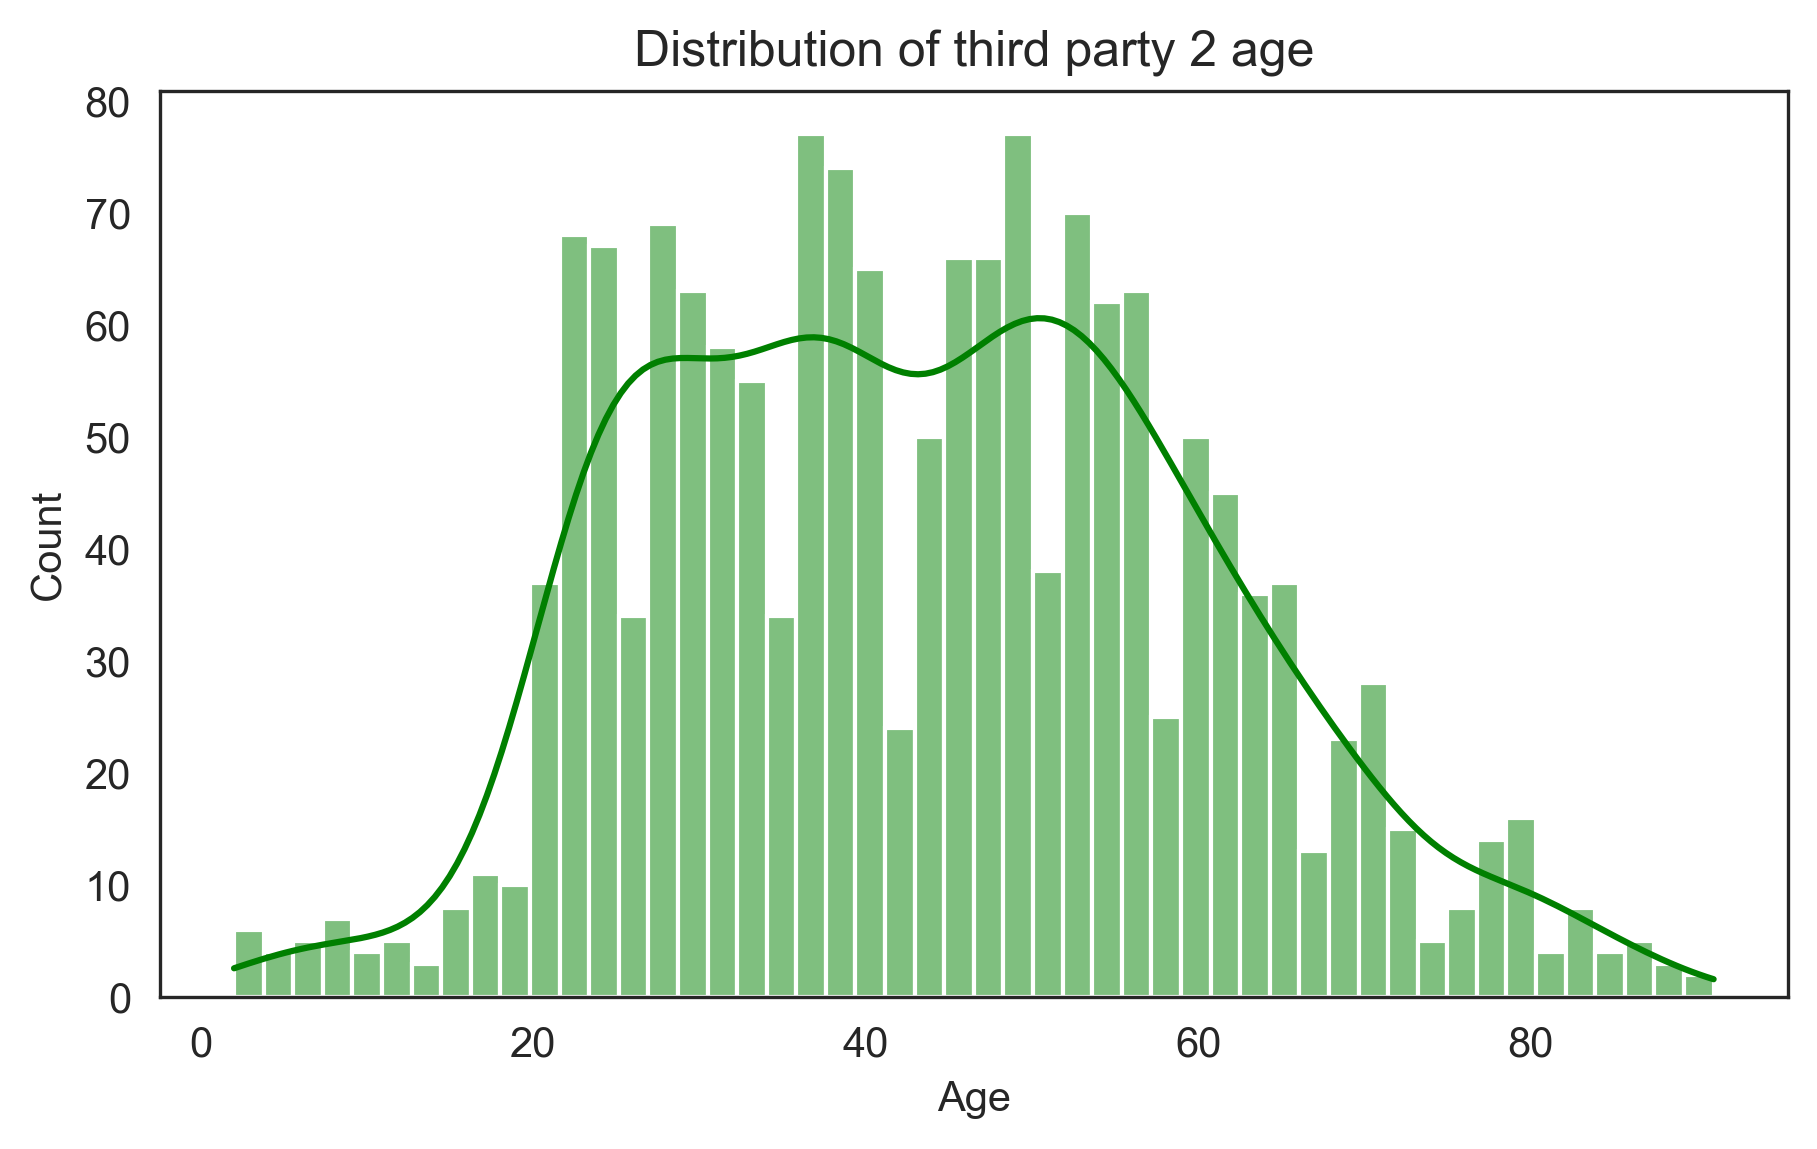
\includegraphics[width=1\linewidth]{dist_third_party_2_age}
  \label{fig:sub4}
\end{subfigure}
\caption{Histograms for age-related features. Green lines are the kernel density estimates. As third party 3 contains only few non-missing values, its histogram is not shown here.}
\label{fig:feature_engineering_age}
\end{figure}

For time features i.e. \texttt{claim\_time\_occured}, it contains about 88.4\% of missing values and has a format of \texttt{HH:MM}. Therefore, \texttt{claim\_time\_occured} is binned in terms of hours, 00:00-01:00, 01:00-02:00,..., 23:00-24:00, and missing values are encoded as \textit{unknown}. Under this categorization, non-missing time can be kept as a feature. Other binning schemes are possible but it is natural to bin time with \texttt{HH:MM} format into hours.\\  

The dataset contains features related to the postal code, including \texttt{claim\_postal\_code}, \texttt{policy\_\\holder\_postal\_code}, \texttt{driver\_postal\_code}, \texttt{third\_party\_1\_postal\_code}, \texttt{third\_party\_2\_\\postal\_code}, \texttt{third\_party\_3\_postal\_code}and \texttt{repair\_postal\_code}. However, these features have more than 1,000 unique postal code values. Without data binning, one hot encoding will create sparse data matrix and greatly increase the dimension of dataset. To avoid a huge search space, we keep the postal codes by their information values, calculated from their weights of evidence. For imbalanced data, we considered a lower threshold for information value, and the postal codes are preserved when their information values are greater than 0.01. Otherwise, they will be grouped under the same level, namely, \textit{other} because they do not contribute much to detect fraudulent cases. A small threshold of 0.01 is used because there are many factor levels.  The results are summarized in exploratory data analysis section.\\

\begin{table}[h]
	\centering
	\begin{tabular}{|l|c|}
	\hline
	Postal code-related features & Number of distinct values \\
	\hline
	\texttt{claim\_postal\_code} & 1060 \\
	\texttt{policy\_holder\_postal\_code} & 1082 \\
	\texttt{driver\_postal\_code} & 1077 \\
	\texttt{third\_party\_1\_postal\_code} & 1088 \\
	\texttt{third\_party\_2\_postal\_code} & 750 \\
	\texttt{third\_party\_3\_postal\_code} & 27 \\
	\texttt{repair\_postal\_code} & 754 \\
	\hline
	\end{tabular}
	\caption{Total number of distinct postal codes for each related feature in the dataset}
\end{table}

Apart from postal code, \texttt{policy\_coverage\_type} also have many factor levels. So, weight of evidence encoding is applied for the similar reason. For other techniques, the odds-based grouping also provides similar results whereas one-dimensional k-means is only applicable to continuous features. Grouping postal code by frequency seems a less plausible method for imbalanced dataset because the grouping may be biased to the majority class. Hence, weight of evidence encoding is a good method in our case. \\

There are some id-related features in the dataset, for instance, \texttt{claim\_vehicle\_id}, \texttt{policy\_hold\\er\_expert\_id}, \texttt{third\_party\_1\_id}, \texttt{third\_party\_1\_vehicle\_id} and \texttt{third\_party\_1\_expert\_id}. As every id-related feature is anonymized, one hot encoding may also lead to a huge increase in dimension. Dummy encoding of id-related features, with known id labelled as 1 and missing id labelled as 0, gives meaningful interpretation to them. 

\subsection*{Exploratory data analysis}
\addcontentsline{toc}{subsection}{Exploratory data analysis}

In the exploratory analysis, most graphs are visualized using \texttt{seaborn} and \texttt{matplotlib} in python. Treemaps are visualized using \texttt{squarify}.

\subsubsection*{Class imbalance problem}
\addcontentsline{toc}{subsubsection}{Class imbalance problem}

Class imbalance problem makes the classification task harder. In the dataset, 55,155 cases are non-fraudulent, and 308 cases are fraudulent which accounts for 0.56\% of the total sample, as summarized in figure 5. There are very few fraudulent cases in the dataset, and hence the dataset is imbalanced. It suggests some sampling techniques e.g. upsampling or smart sampling as well as metrics (other than accuracy) are needed in the training process so as to overcome the class imbalance problem.

\begin{figure}[h]
\centering
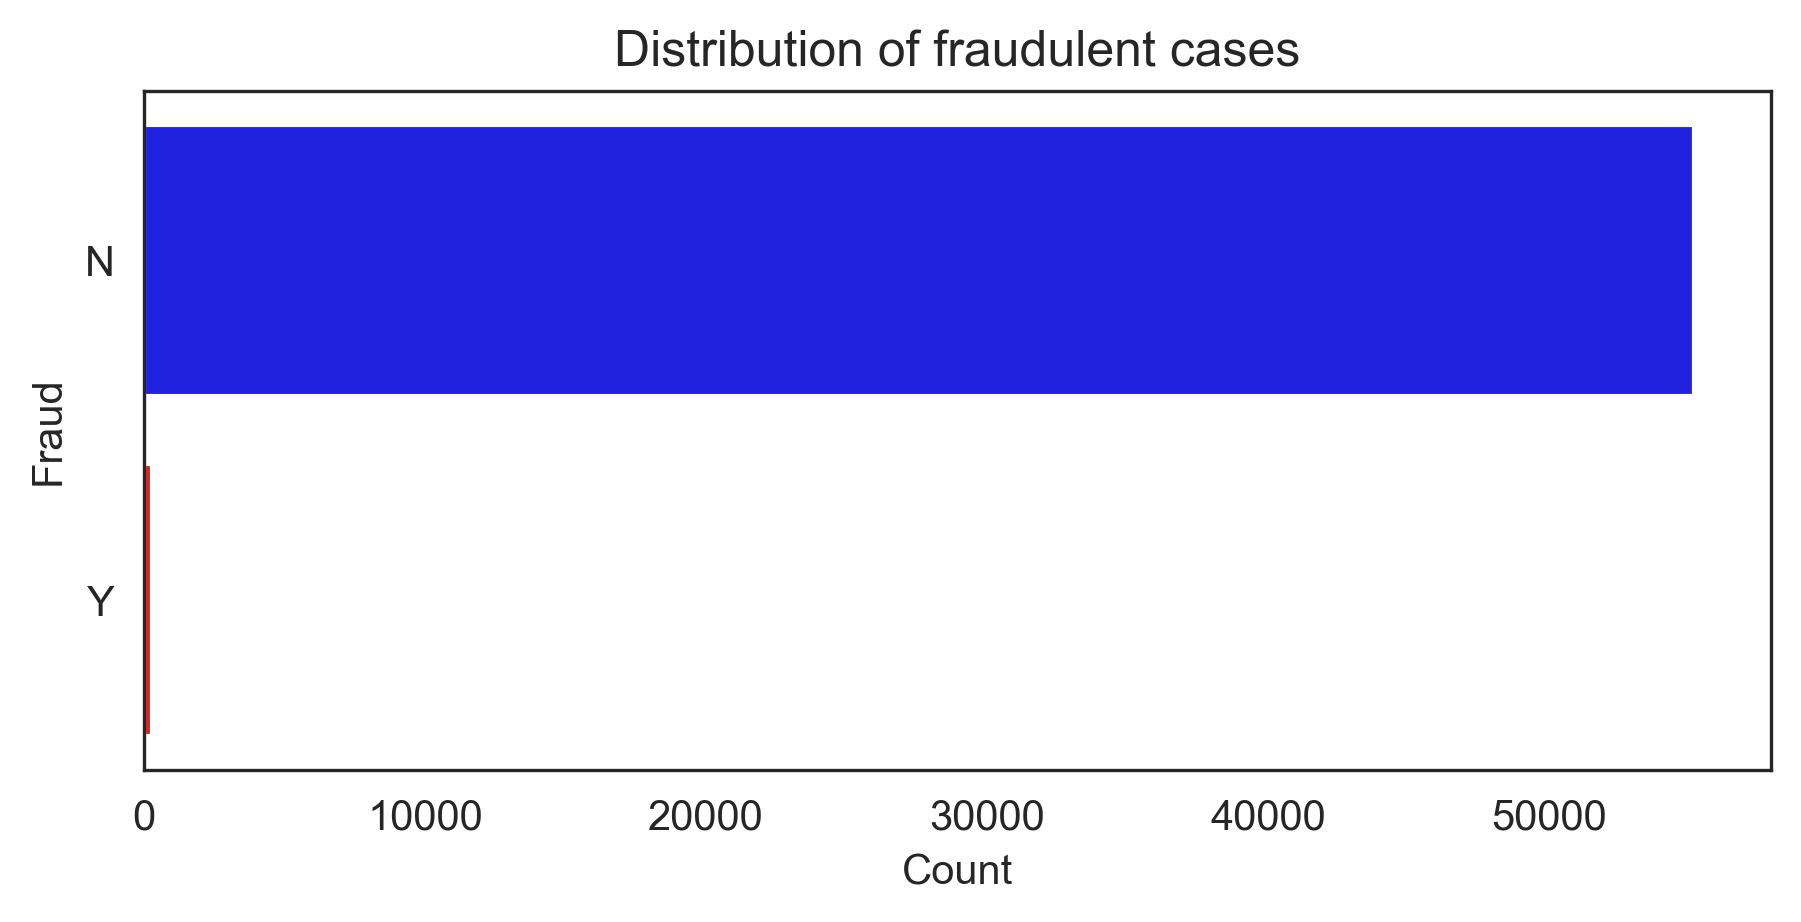
\includegraphics[width = 12cm]{class_imbal_problem}
\caption{Barplot for \texttt{fraud}}
\end{figure}

\vspace{-1cm}
\subsubsection*{Univariate analysis}
\addcontentsline{toc}{subsubsection}{Univariate analysis}

To develop a basic understanding of the training data, some features are covered in the univariate analysis. The feature \texttt{claim\_amount} is only provided in the training data which serves as a weighting variable in scoring because the goal of the classification task is to predict the probabilities of top 100 fraudulent cases in terms of their insurance claim amounts. We observe the distribution for \texttt{claim\_amount} is highly right-skewed. Some observations have very high claiming amounts. In general, fraudulent cases tend to have higher claim amounts as their median and the upper quartile are much higher than those of non-fraudulent cases. Still, there are some non-fraudulent cases having high claim amounts. 

\begin{figure}[h]
\centering
\begin{subfigure}{.5\textwidth}
  \centering
  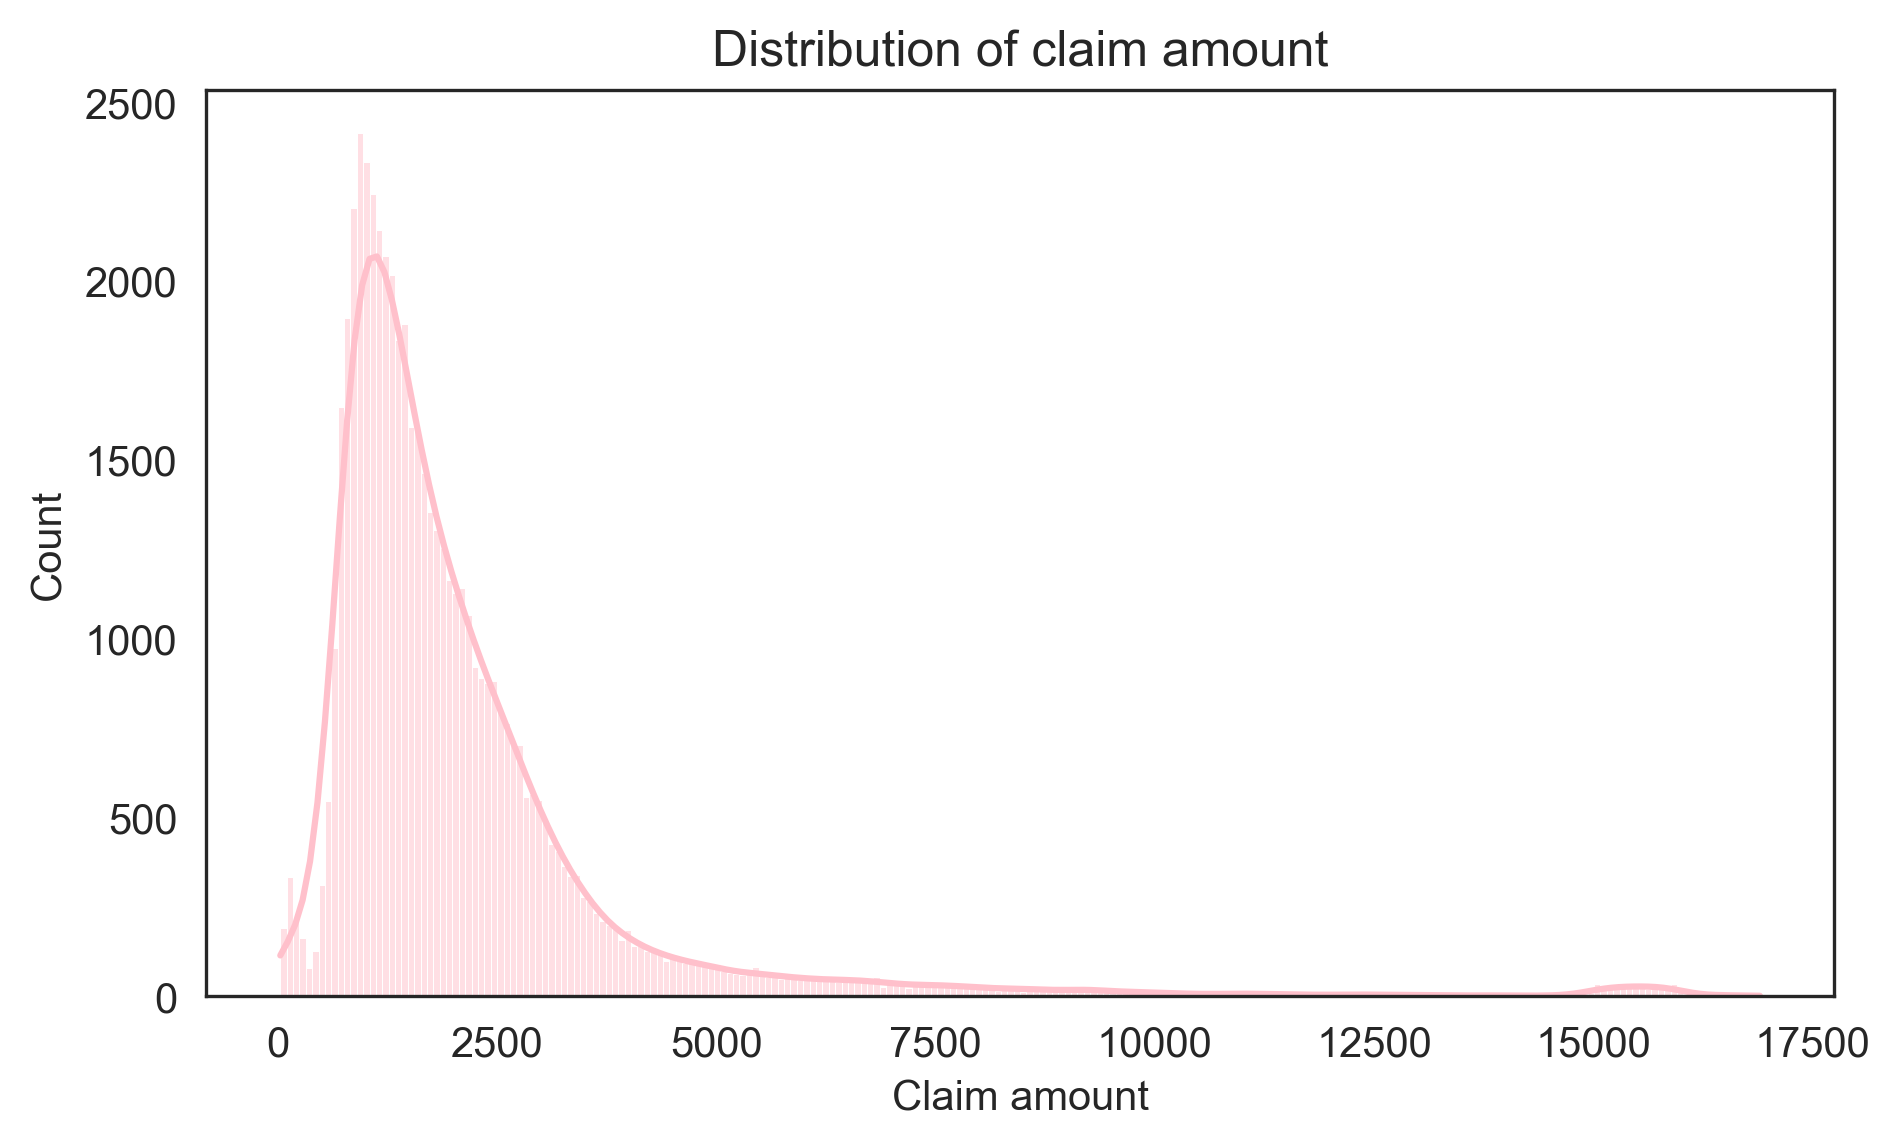
\includegraphics[width=1\linewidth]{dist_claim_amount}
  \label{fig:sub1}
\end{subfigure}%
\begin{subfigure}{.5\textwidth}
  \centering
  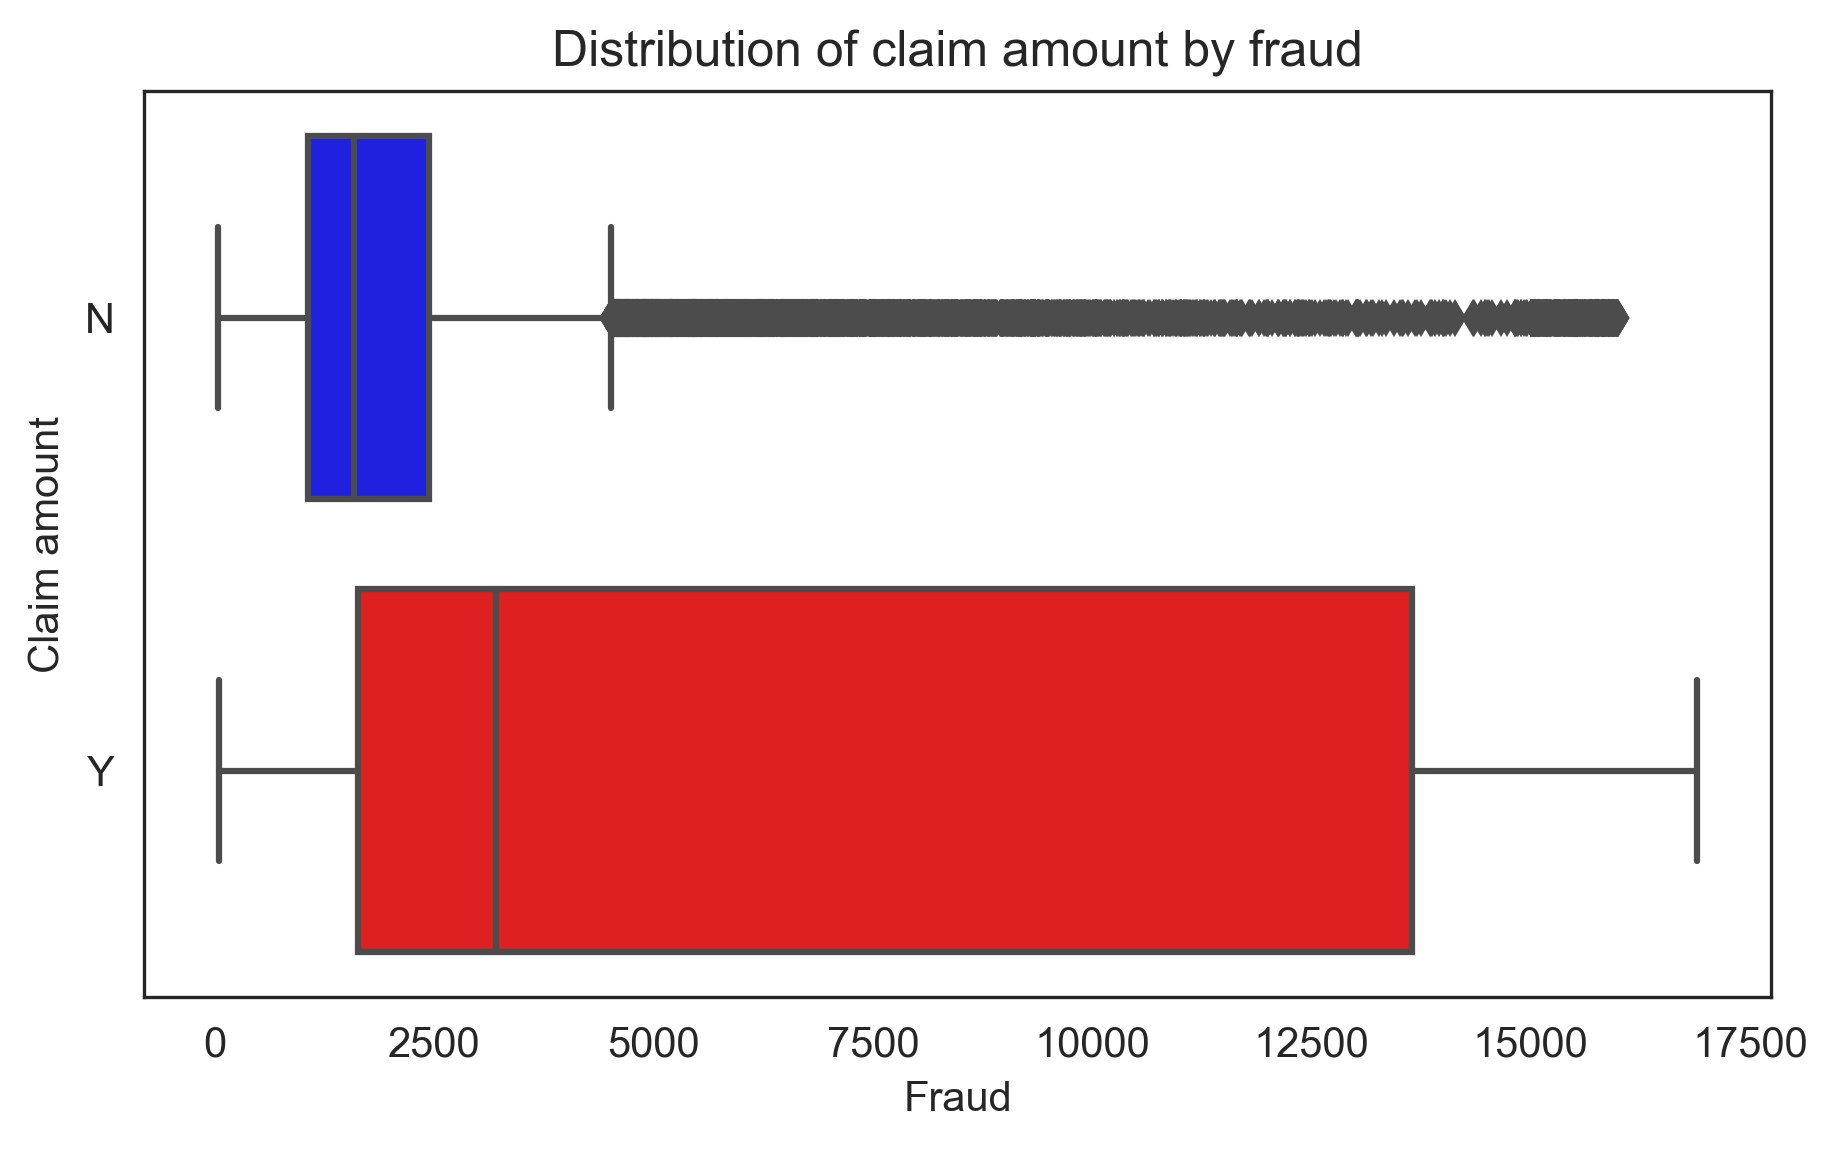
\includegraphics[width=1\linewidth]{dist_claim_amount_by_fraud}
  \label{fig:sub2}
\end{subfigure}
\caption{Distribution of \texttt{claim\_amount}}
\label{fig:test}
\end{figure}

The dataset contains some features related to the third parties, and \texttt{claim\_num\_third\_party} indicates the number of third parties involved. There are about 69\% of cases involved exactly one third party. About 24.7\% of cases do not involve any third party, and only 6.3\% of cases involve more than one third party. The average claim amounts and frequency of the number of third party conditioned on fraudulent status are summarized as heatmaps presented in figure 7. For fraudulent cases, about 58\% of observations do not have third party, and 39\% of them have one third party. Unlike non-fraudulent cases, about 69\% of observations have one third party and only 25\% of them have no third party. However, in terms of average claim amounts, fraudulent cases have high values for instances with more than one third party. It means features related to the second and the third third parties may be useful in classification.

\begin{figure}[h]
\centering
\begin{subfigure}{.6\textwidth}
  \centering
  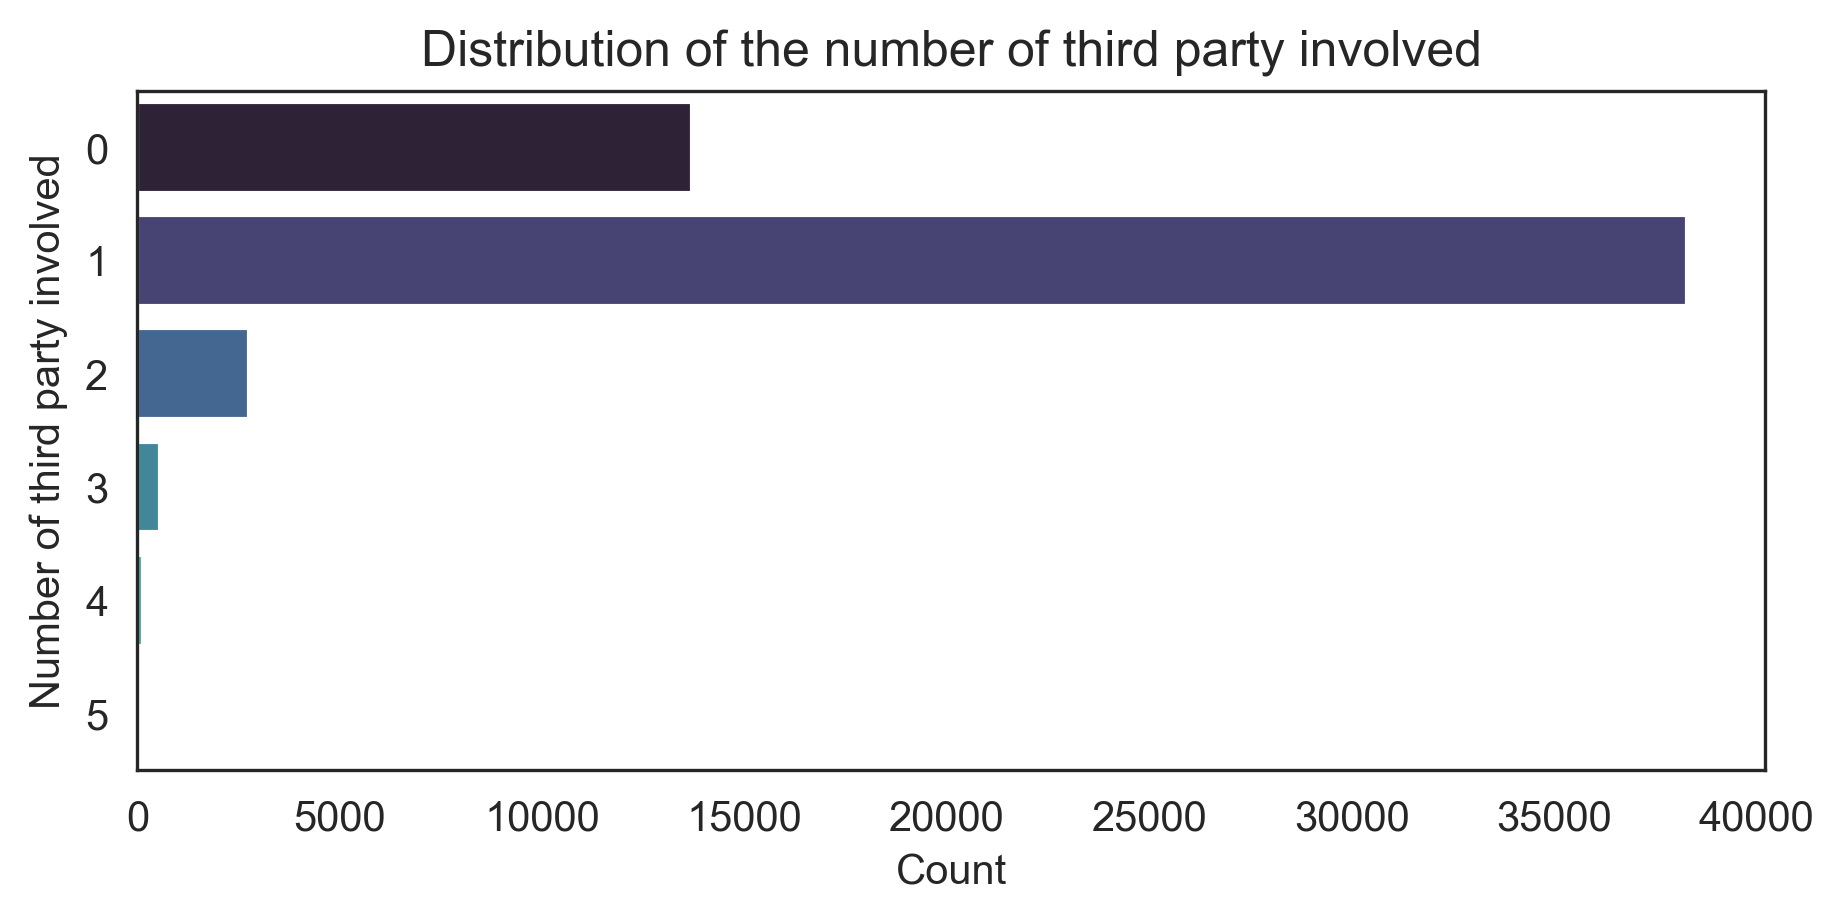
\includegraphics[width=1\linewidth]{num_third_party_involved}
  \label{fig:sub1}
\end{subfigure}%
\begin{subfigure}{.4\textwidth}
  \centering
  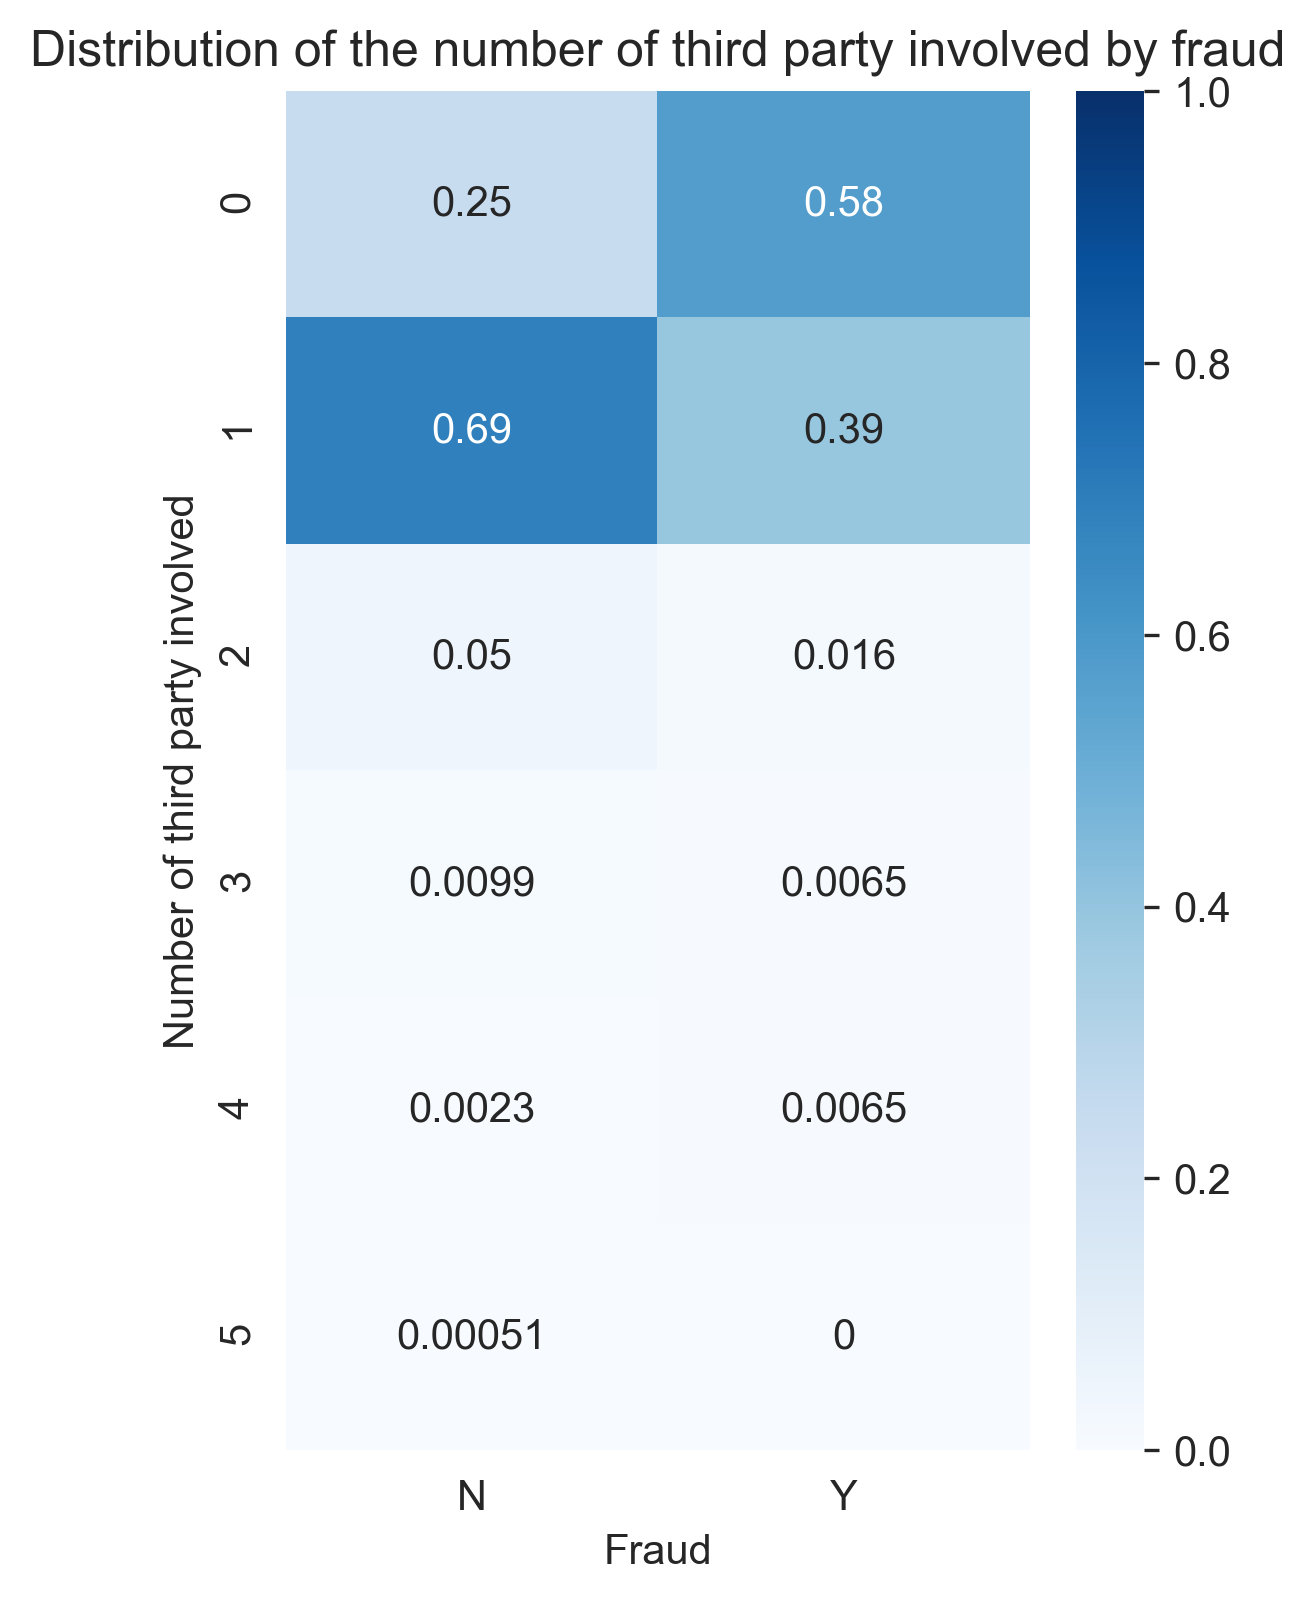
\includegraphics[width=1\linewidth]{num_third_party_involved_by_fraud}
  \label{fig:sub2}
\end{subfigure}
\begin{subfigure}{0.7\textwidth}
  \centering
  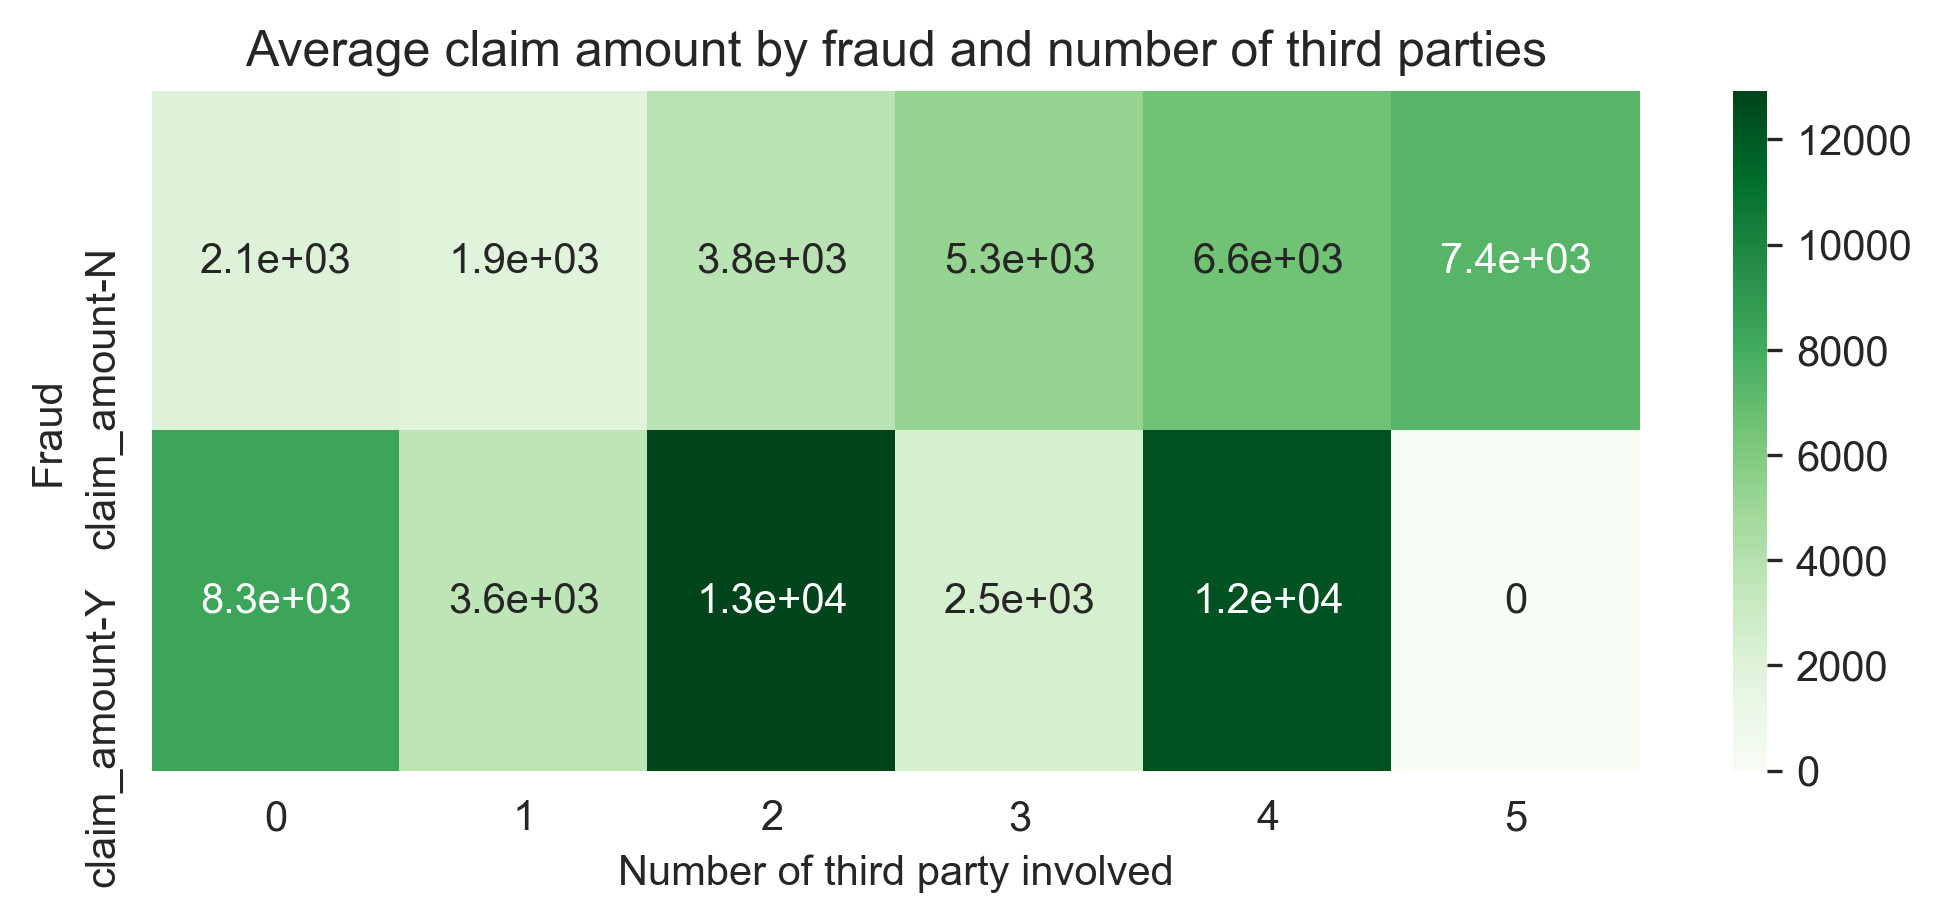
\includegraphics[width=1\linewidth]{num_third_party_involved_by_fraud2}
  \label{fig:sub2} 
\end{subfigure}
\caption{Distributions of \texttt{claim\_num\_third\_parties} with barplot and heatmaps}
\label{fig:eda_third_party_num}
\end{figure}

To know whether the occurrence of fraudulent cases and their claim amounts vary across vehicle brands, we visualize \texttt{claim\_vehicle\_brand} using treemaps from \texttt{squarify} library in python. In figure 8, it is clear that vehicles from Porsche, Land Rover and Toyota have the highest average claiming amounts for fraudulent cases. The average claiming amounts are \$15,861 for Porsche, \$15,328 for Land Rover and \$11,640 for Toyota. However, most of the fraudulent cases do not have vehicle brands recorded, which are labelled as \textit{unknown} in figure 9. Apart from missing cases, BMW, Volkswagen and Citroen are found to be most frequent fraudulent cases. \\

Among various claim causes, we found that \textit{fire} and \textit{theft} are associated with higher claim amounts. The most frequent causes for fraudulent cases are \textit{traffic accident}, \textit{theft} and \textit{other}. In the training data, there are only few observations for \textit{windows}, \textit{weather} and \textit{vandalism}. The violinplot in figure 10 summarizes the findings. 

\begin{figure}[h]
\centering
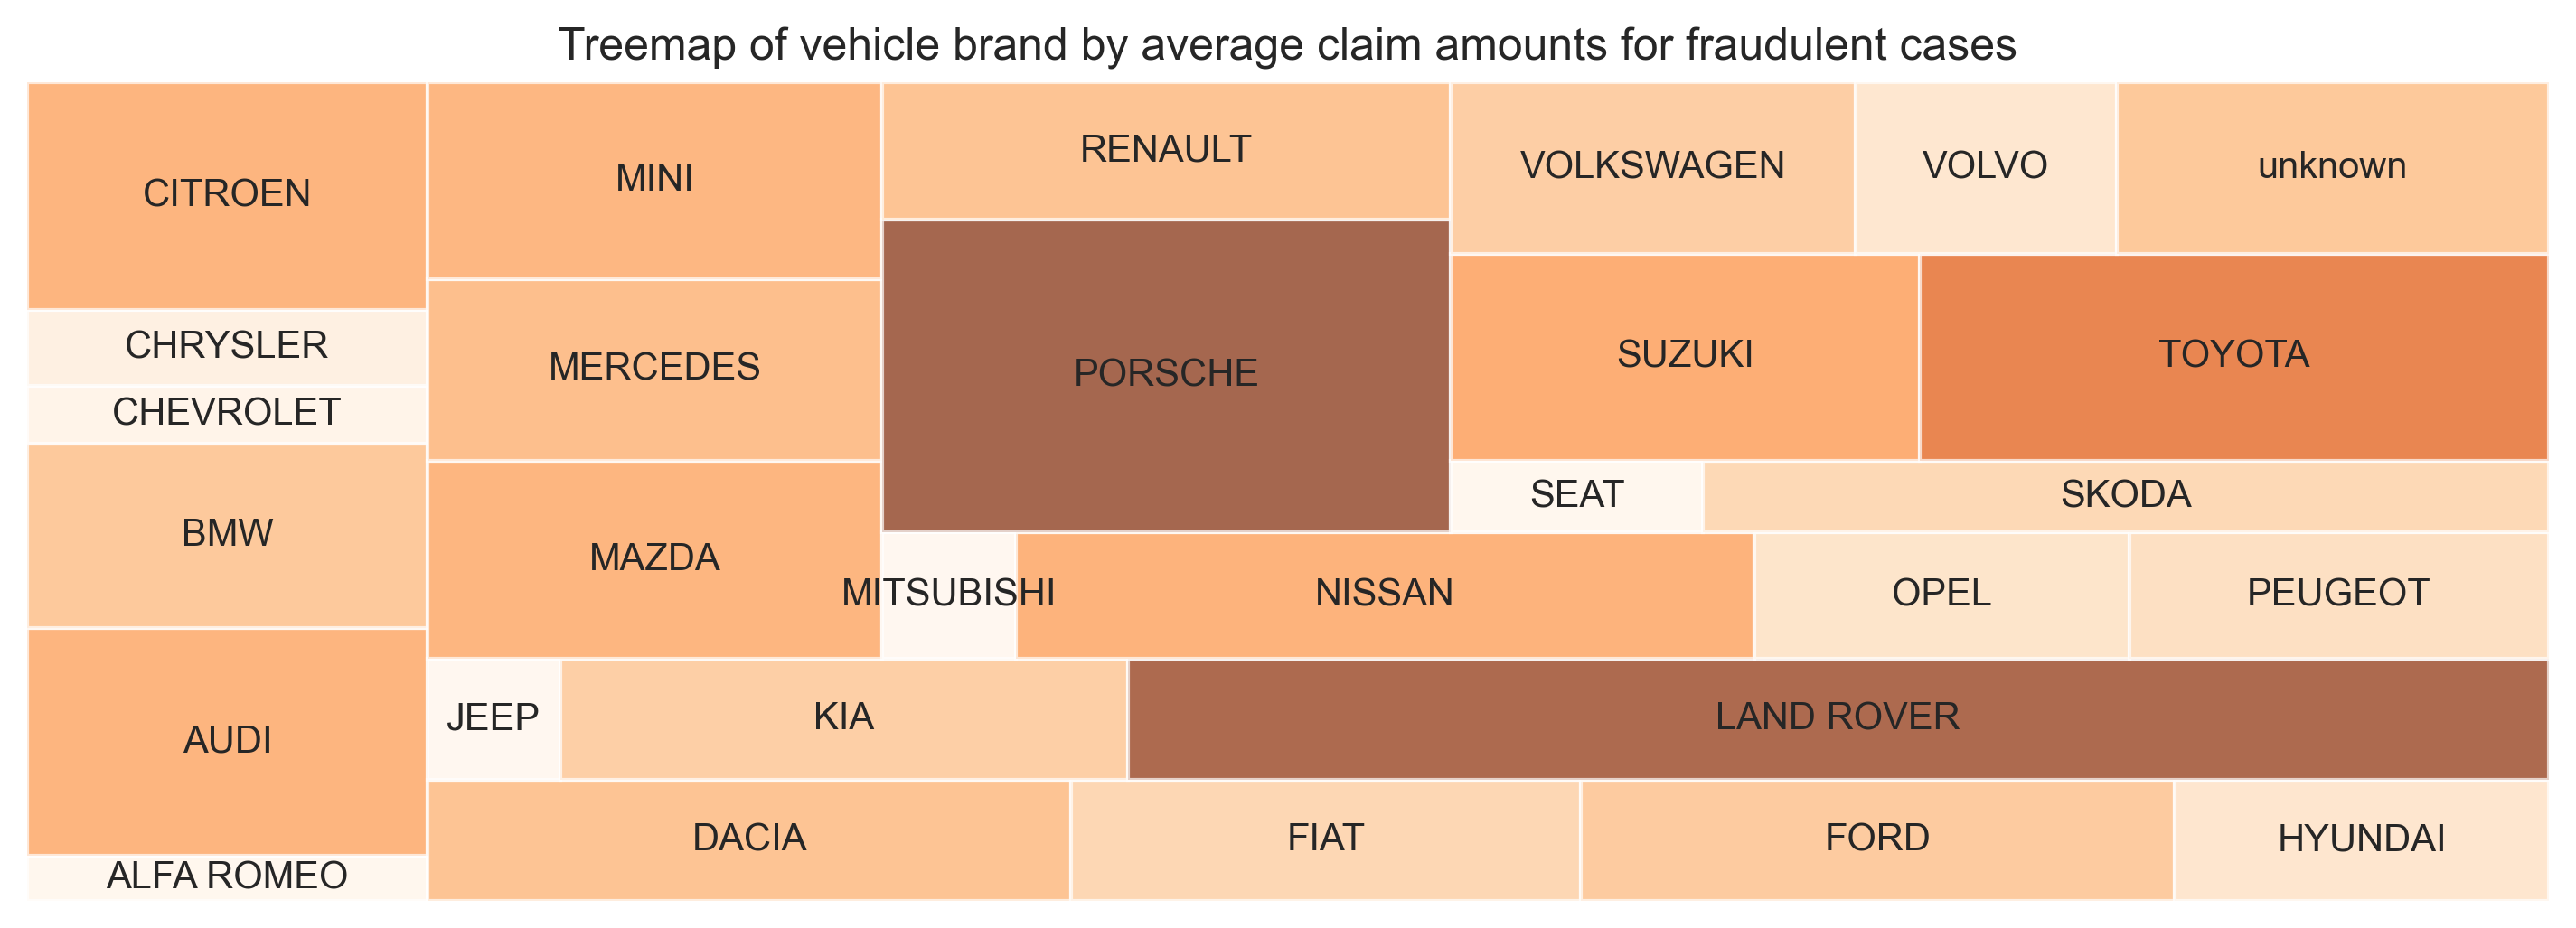
\includegraphics[width = 13cm, height = 6cm]{treemap_vehicle_brand_average_claim_amount}
\caption{Average claim amounts of fraudulent cases for different vehicle brands}
\vspace{0.5cm}
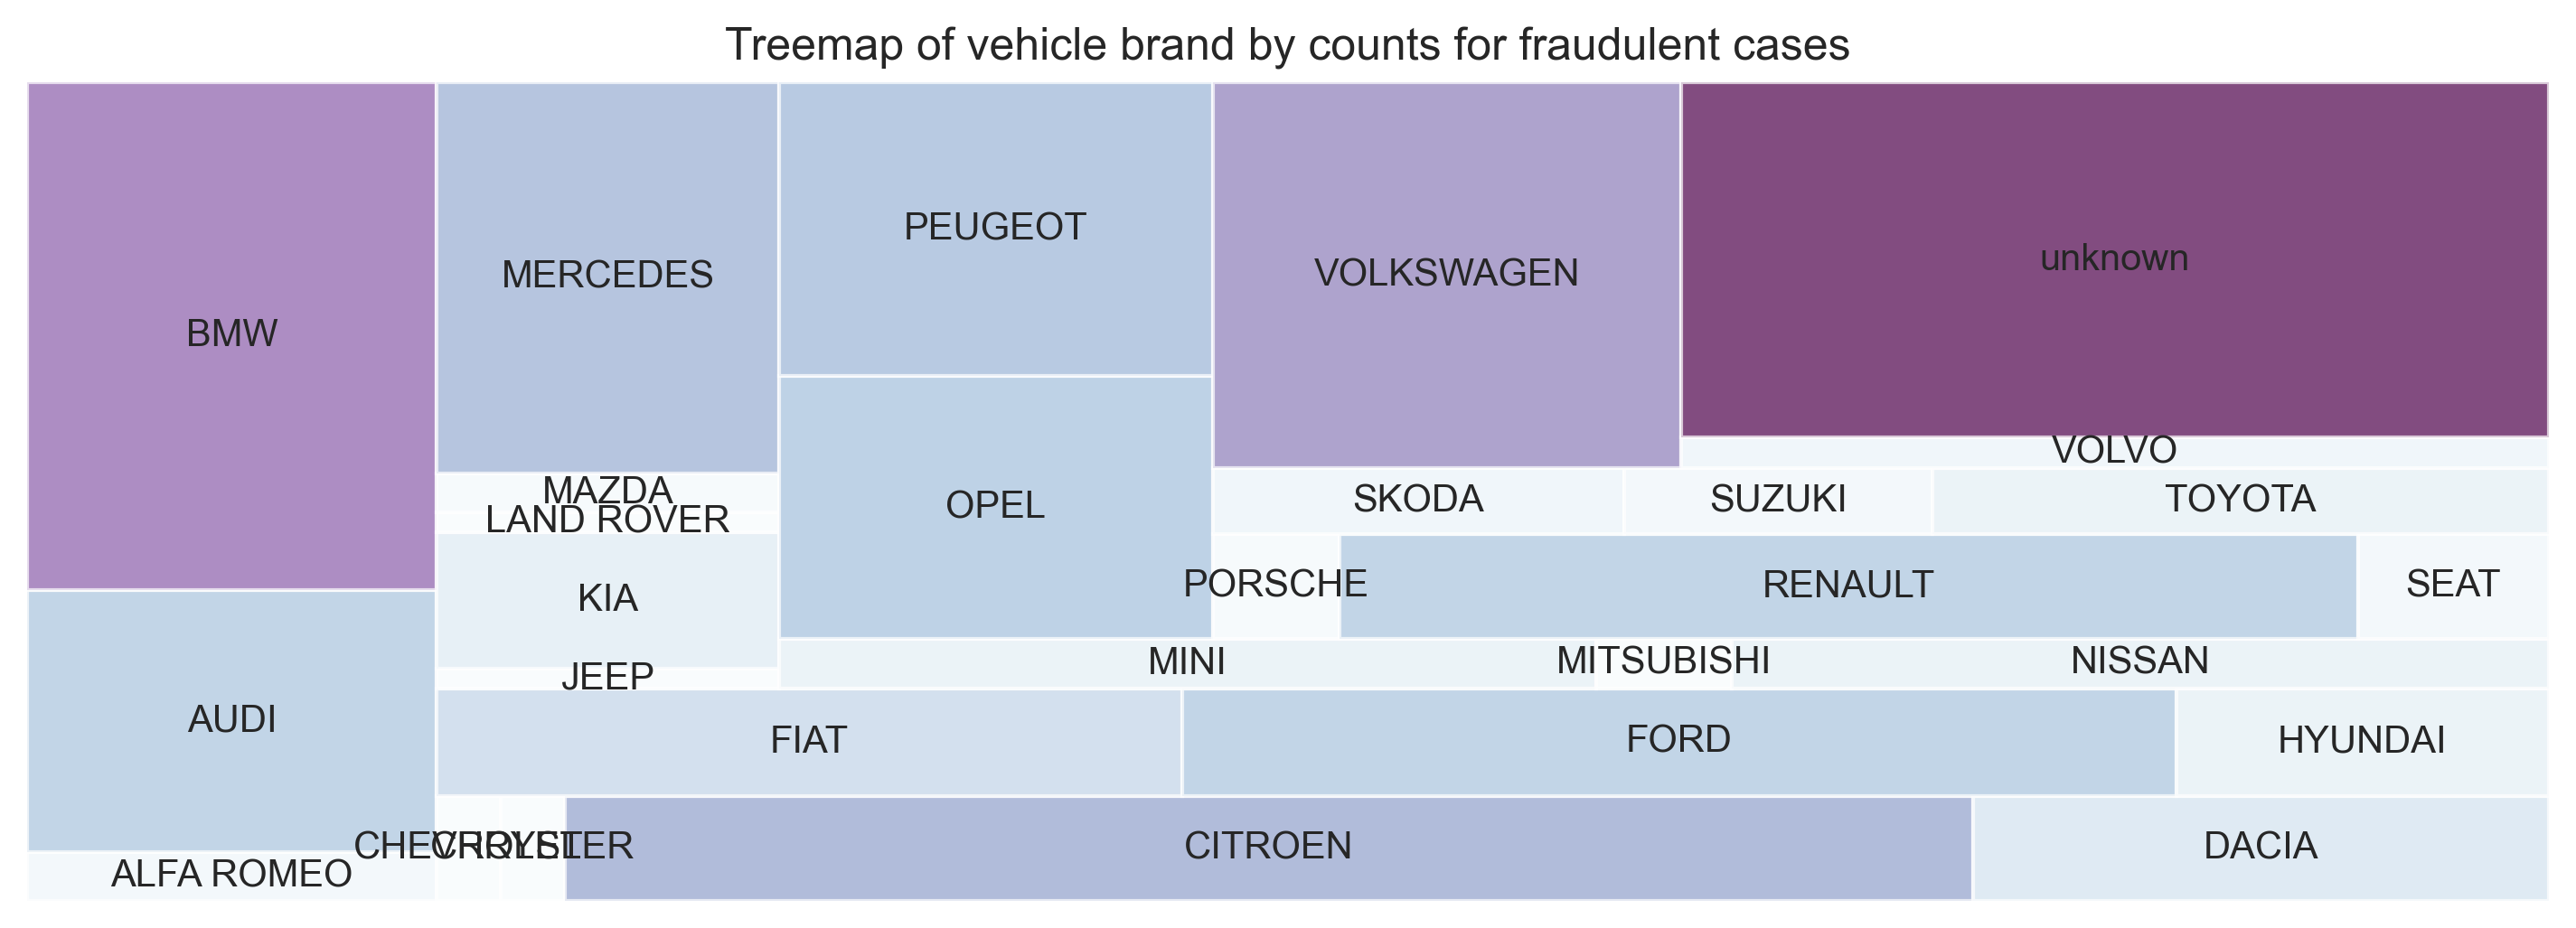
\includegraphics[width = 13cm, height = 6cm]{treemap_vehicle_brand_count}
\caption{Counts of fraudulent cases for different vehicle brands}
\vspace{0.5cm}
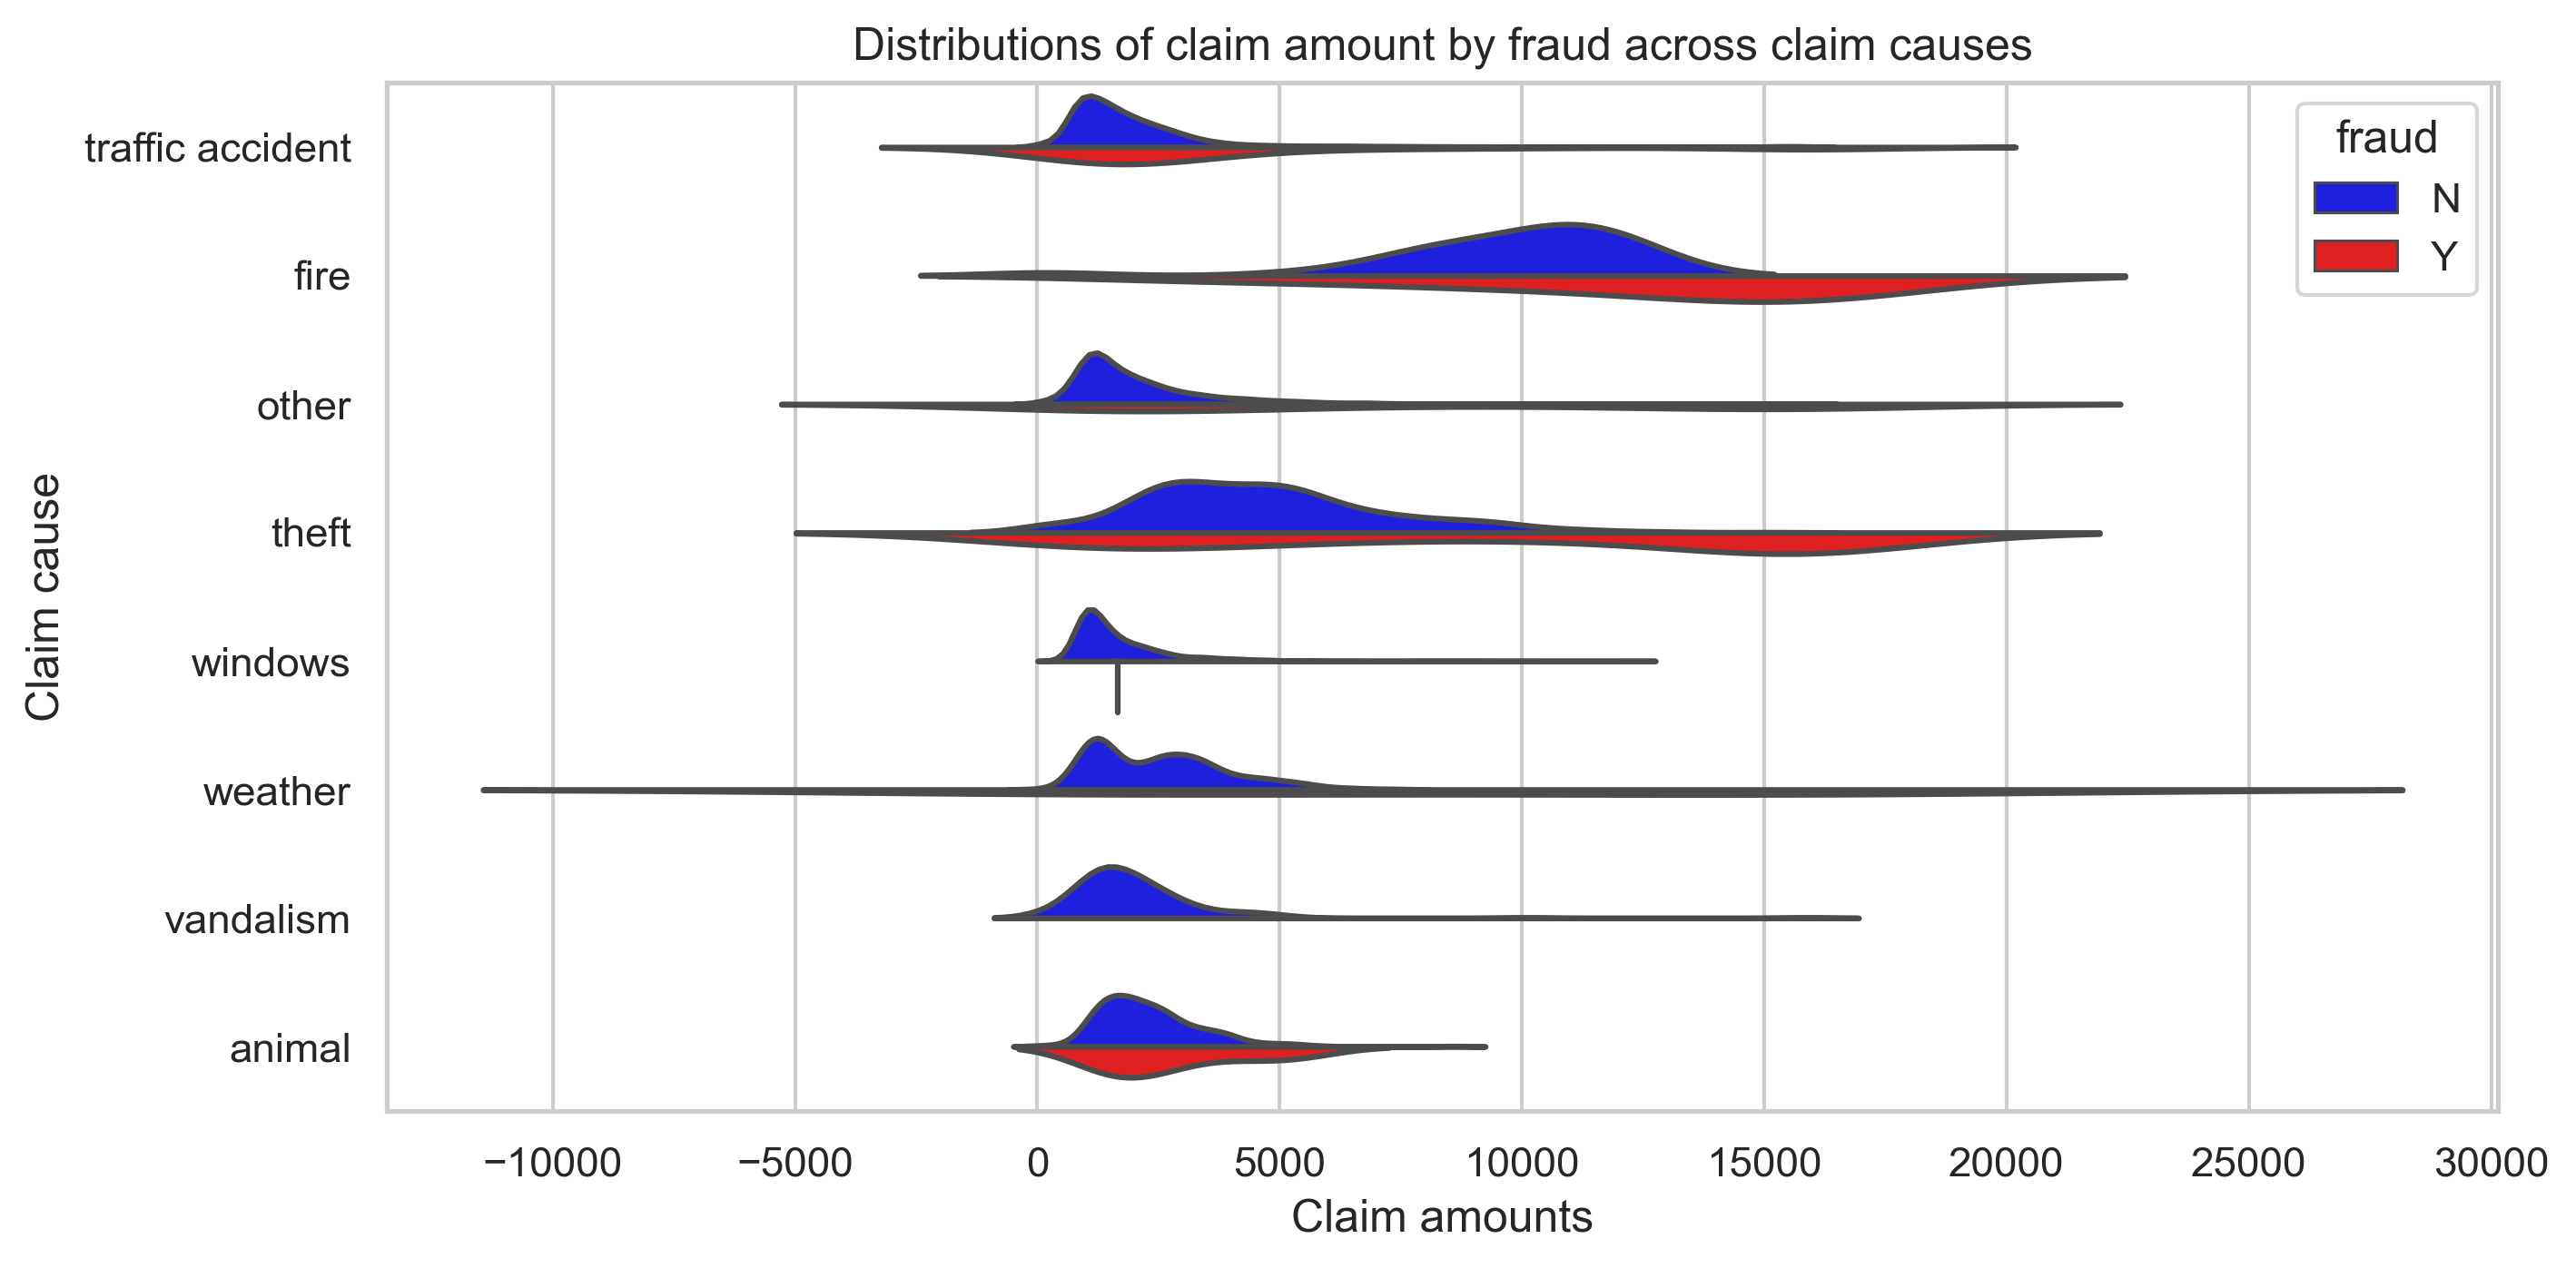
\includegraphics[width = 14cm, height = 9cm]{violin_plt_claim_amt_by_fraud_across_causes}
\caption{Distributions of claim amounts by fraudulent status and claim causes}
\end{figure}

\clearpage

\begin{table}
	\begin{tabular}{|c|cccccccc|}
	\hline
	\texttt{claim\_cause} & animal & fire & other & theft & traffic accident & vandalism & weather & windows \\
	\hline
	\texttt{fraud} = N & 334 & 29 & 7379 & 513 & 43366 & 198 & 744 & 2592 \\
	\texttt{fraud} = Y & 10 & 10 & 56 & 97 & 130 & 0 & 4 & 1\\
	\hline
	\end{tabular}
	\caption{Counts by \texttt{fraud} and \texttt{claim\_cause}}
\end{table}

As discussed in previous section, \texttt{claim\_time\_occured} is binned into 24 hours. Therefore, we can analyze the frequency of claim causes in 24 hours in an exploratory way. A heatmap on the frequency of claim causes across time for non-missing data is presented in figure 11. We observe that the claims due to \textit{animal} usually occur at 06:00 - 07:00 and 22:00 - 23:00. The claims due to \textit{fire} occur most frequently at the afternoon (from 16:00 to 18:00). There is no special time pattern for the claims due to \textit{other}. The claims due to \textit{theft} occur most frequently at 03:00-04:00, and the claims due to \textit{traffic accident} occur at the working time period (07:00-21:00). The claims due to \textit{vandalism} usually occur at 10:00-11:00 and 15:00-16:00. The claims due to \textit{weather} usually occur at 16:00-18:00, and the claims due to \textit{windows} usually occur at 12:00-13:00.

\begin{figure}[h]
\centering
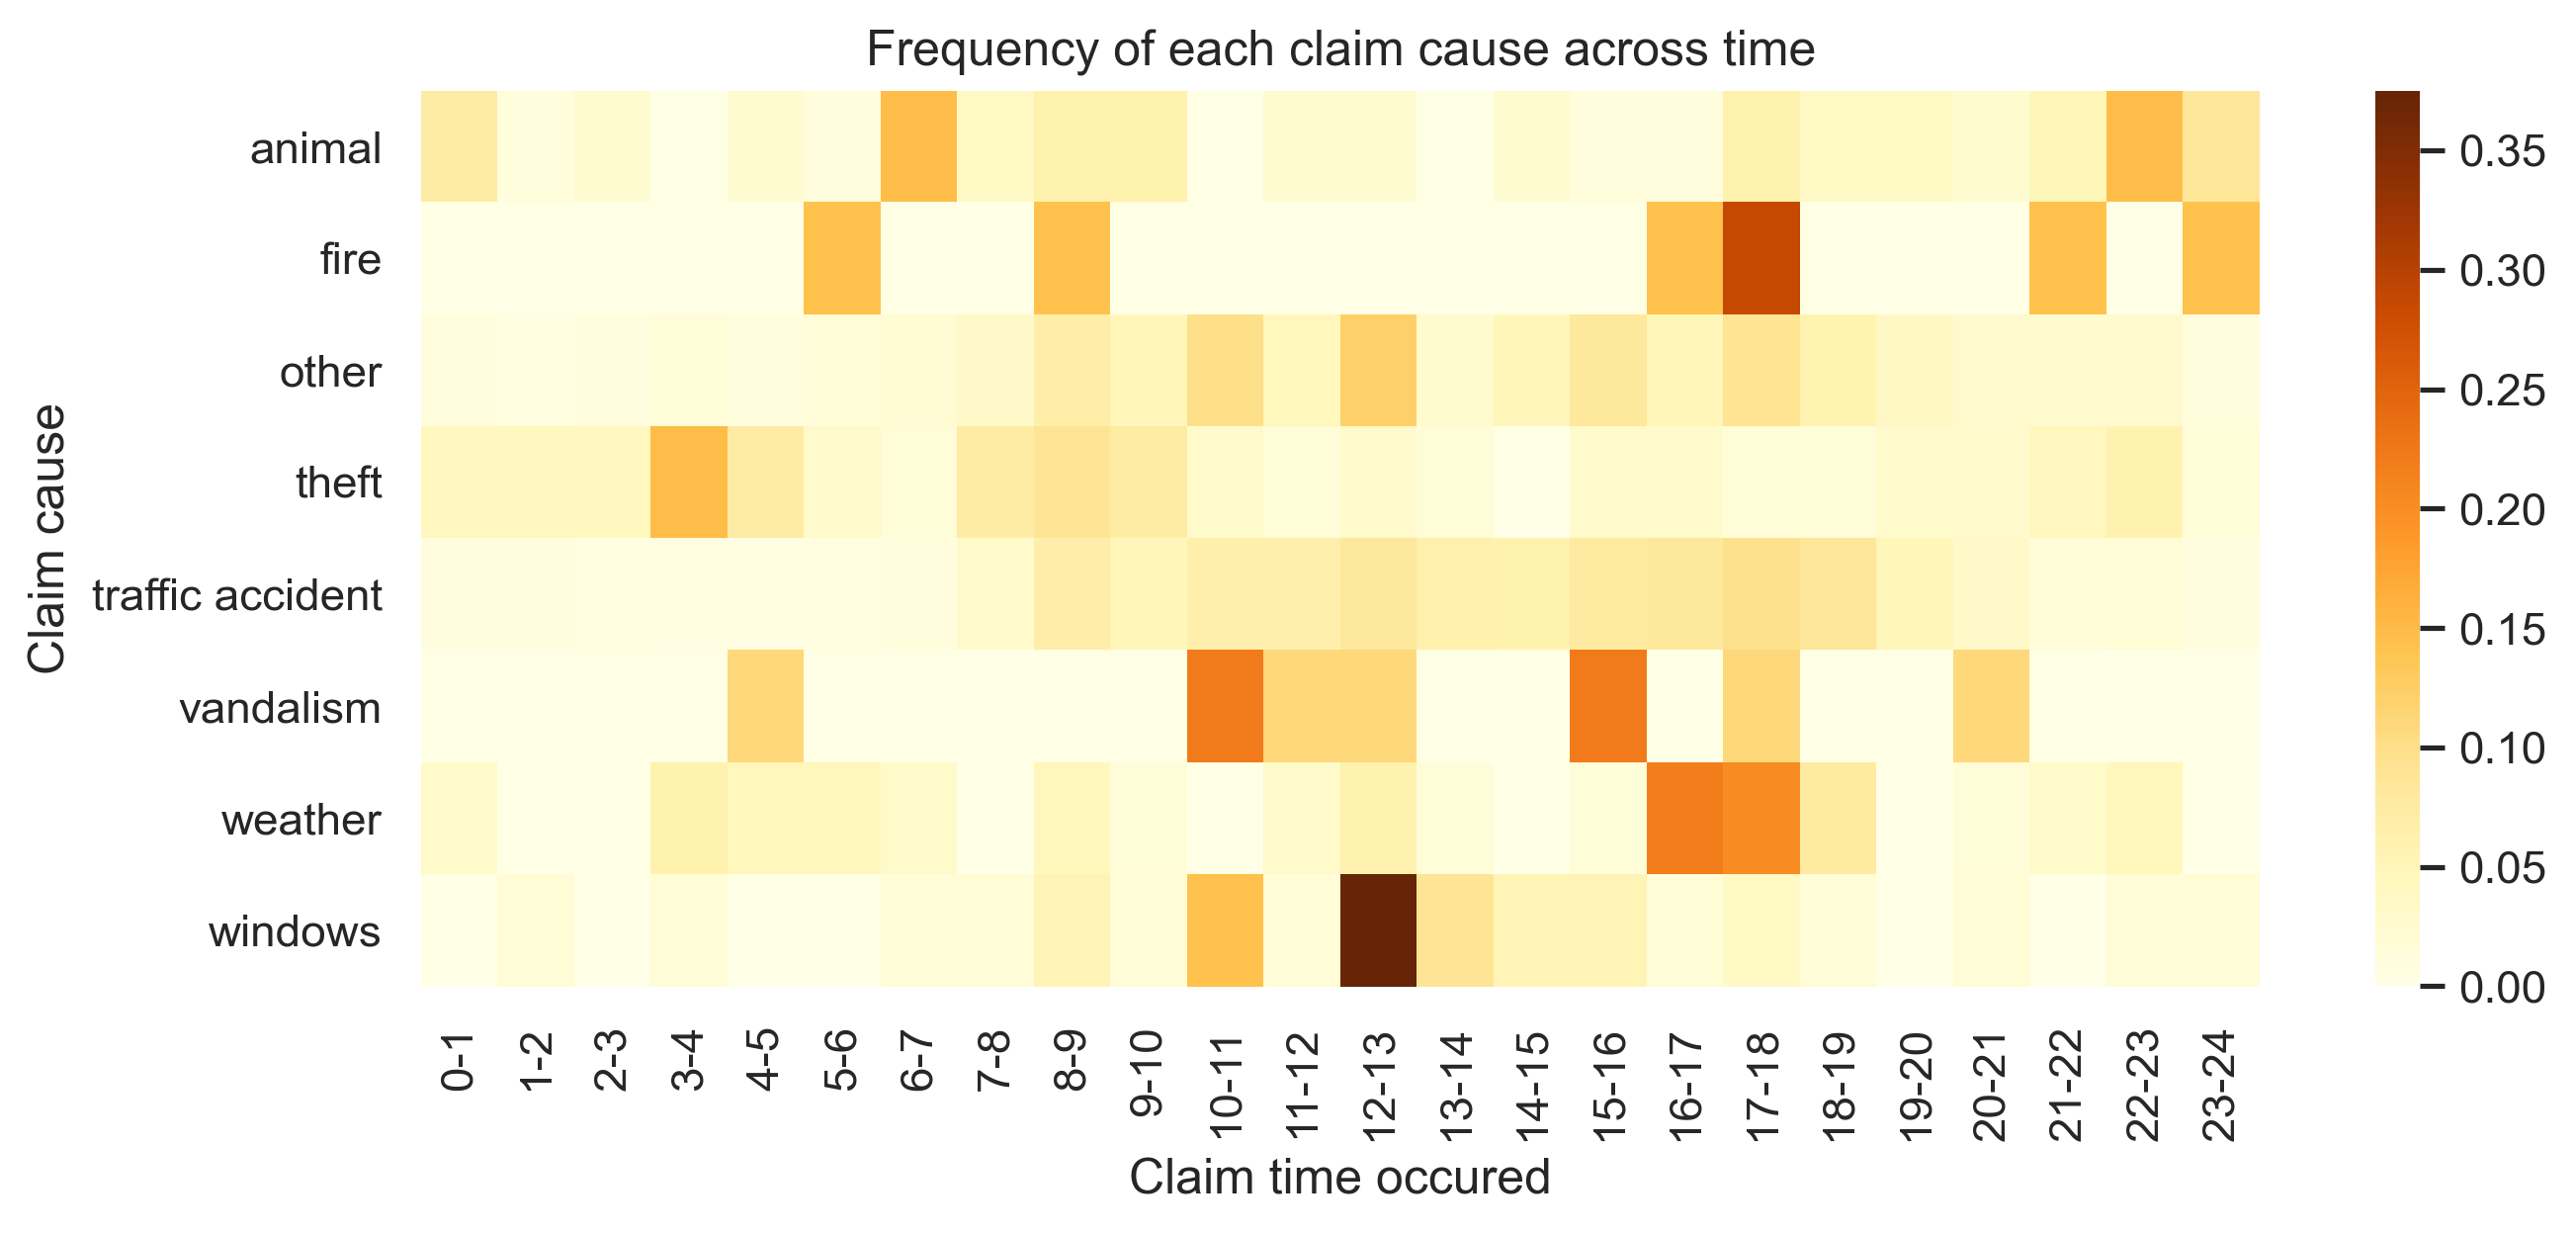
\includegraphics[width = 14cm, height = 7cm]{freq_claim_cause_across_time}
\caption{Frequency of claim causes across time, with missing data excluded}
\end{figure}

For postal code-related features, as discussed in previous section, postal codes are grouped in terms of their information values from the weight of evidence encoding. The corresponding information values are summarized in figure 12. For \texttt{claim\_postal\_code}, postal codes 7700, 1210 and 6030 have relatively high information values. For \texttt{driver\_postal\_code} and \texttt{policy\_holder\_postal\_code}, postal code 7700 also has the highest information values. It seems that postal code 7700 has some evidence for fraudulent cases. For \texttt{repair\_postal\_code}, postal code 1731 has the highest information value. For \texttt{third\_party\_1\_postal\_code}, \textit{unknown} has the highest information value because fraudulent cases mostly have missing values. For \texttt{third\_party\_2\_postal\_code}, postal code 7141 and 3510 have relatively high information values. For \texttt{third\_party\_3\_postal\_code}, there are no fraudulent cases with non-missing values. Therefore, it is not presented here. \\

There are 73 different policy coverage types in total. After weight of evidence encoding, coverage types \#000110000, \#111110001 and \#000110100 show relatively high information values. These coverage types may be informative in identifying fraudulent cases.

\clearpage
\begin{figure}[h]
\centering
\begin{subfigure}{.5\textwidth}
  \centering
  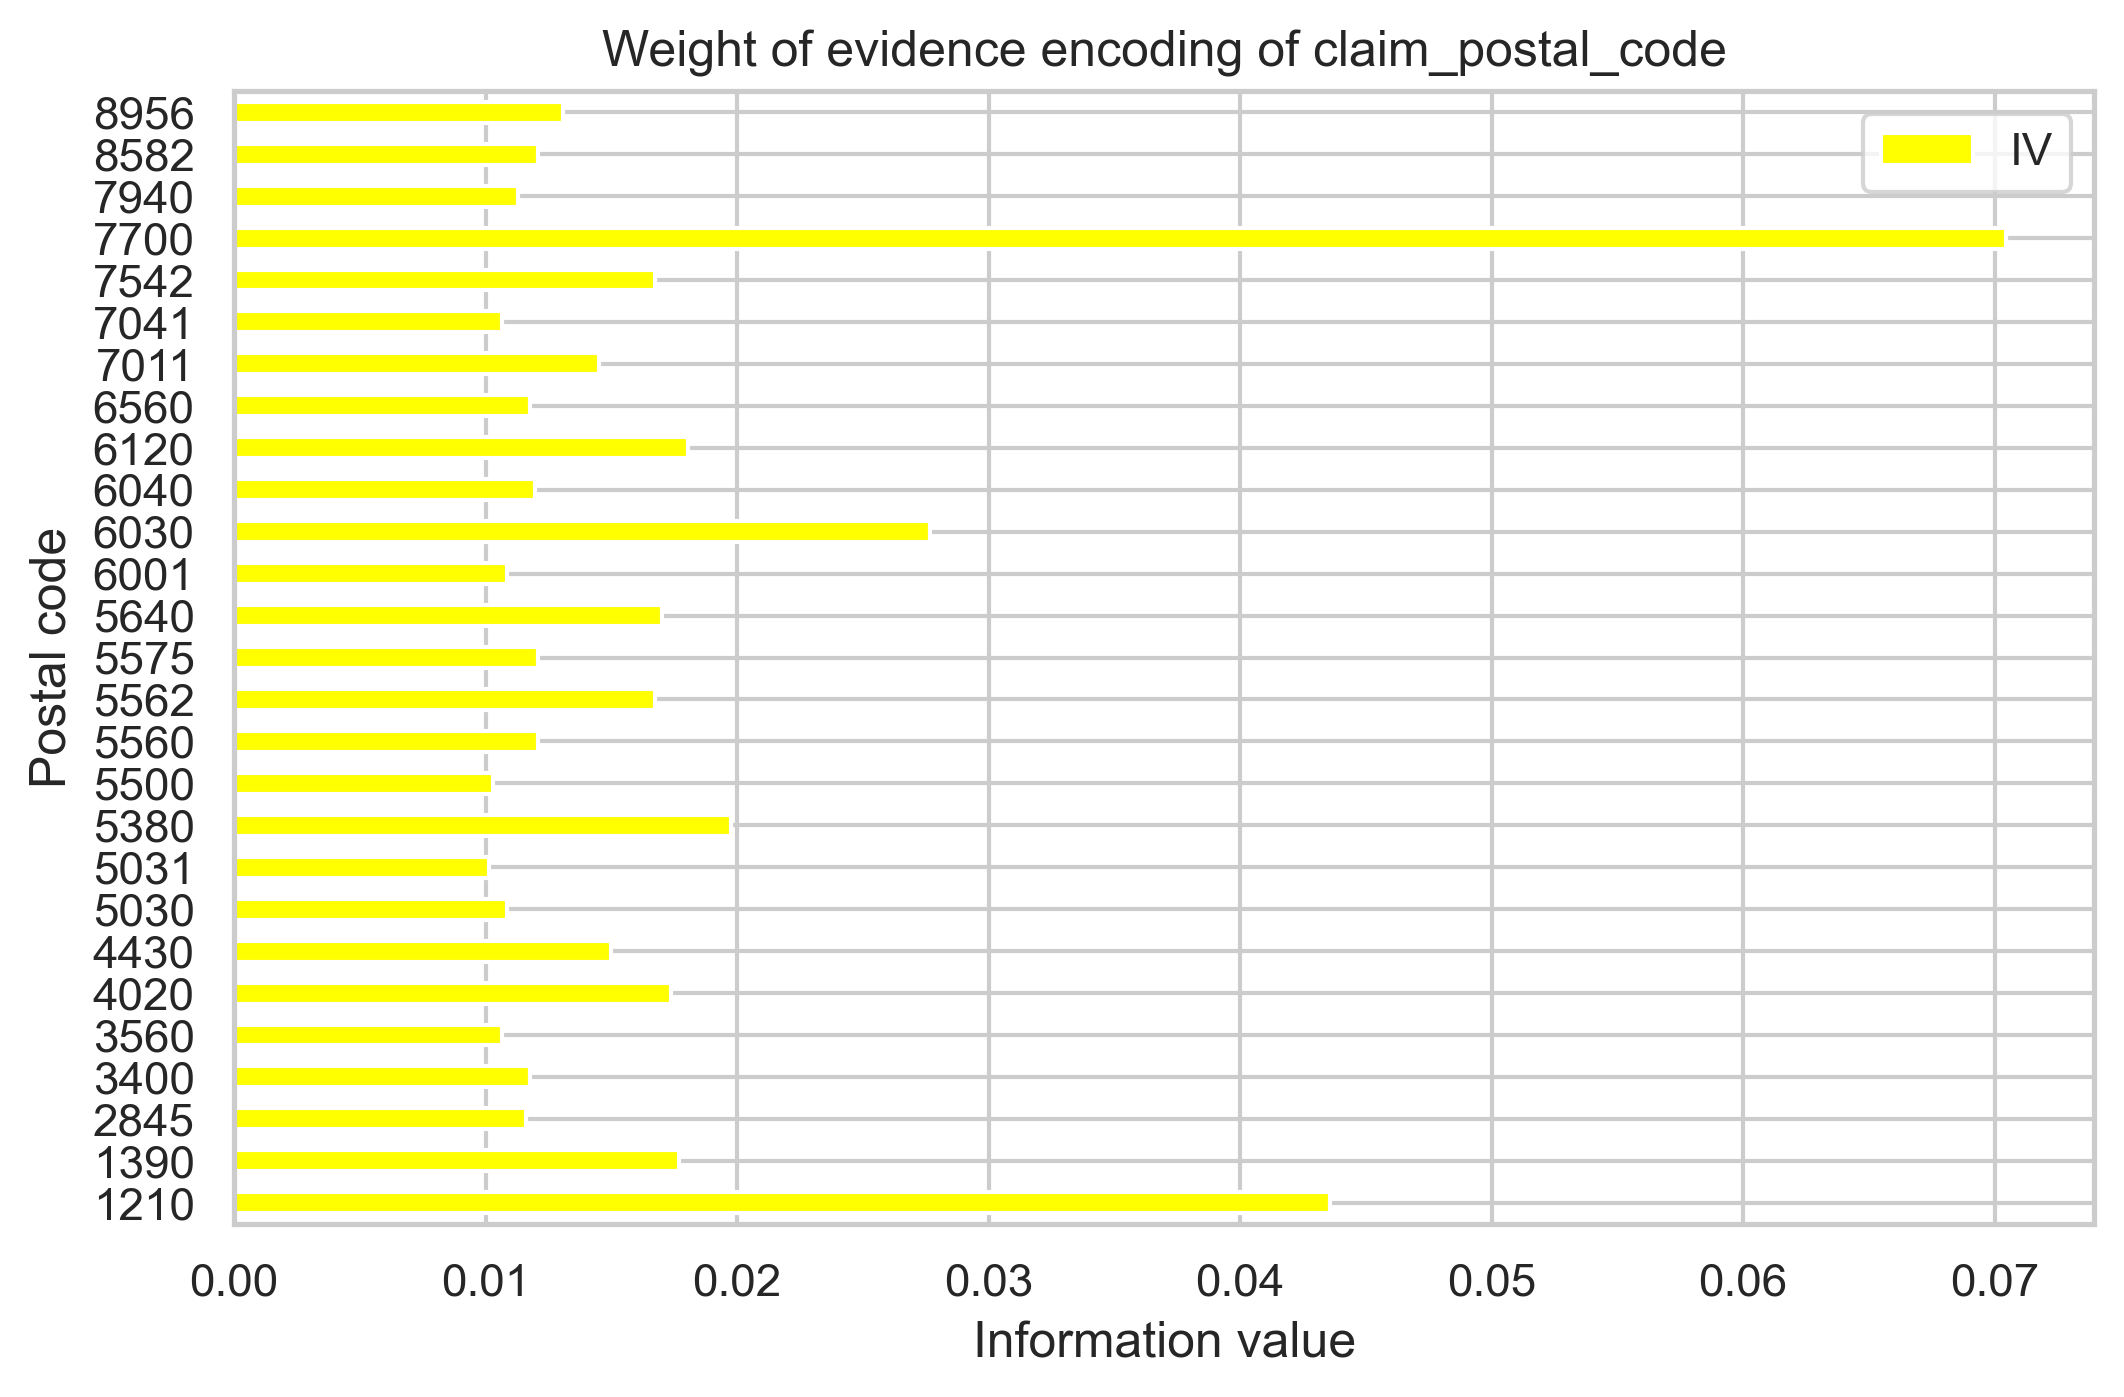
\includegraphics[width=1\linewidth]{info_val_claim_postal_code}
  \caption{\texttt{claim\_postal\_code}}
  \label{fig:sub1}
\end{subfigure}%
\begin{subfigure}{.5\textwidth}
  \centering
  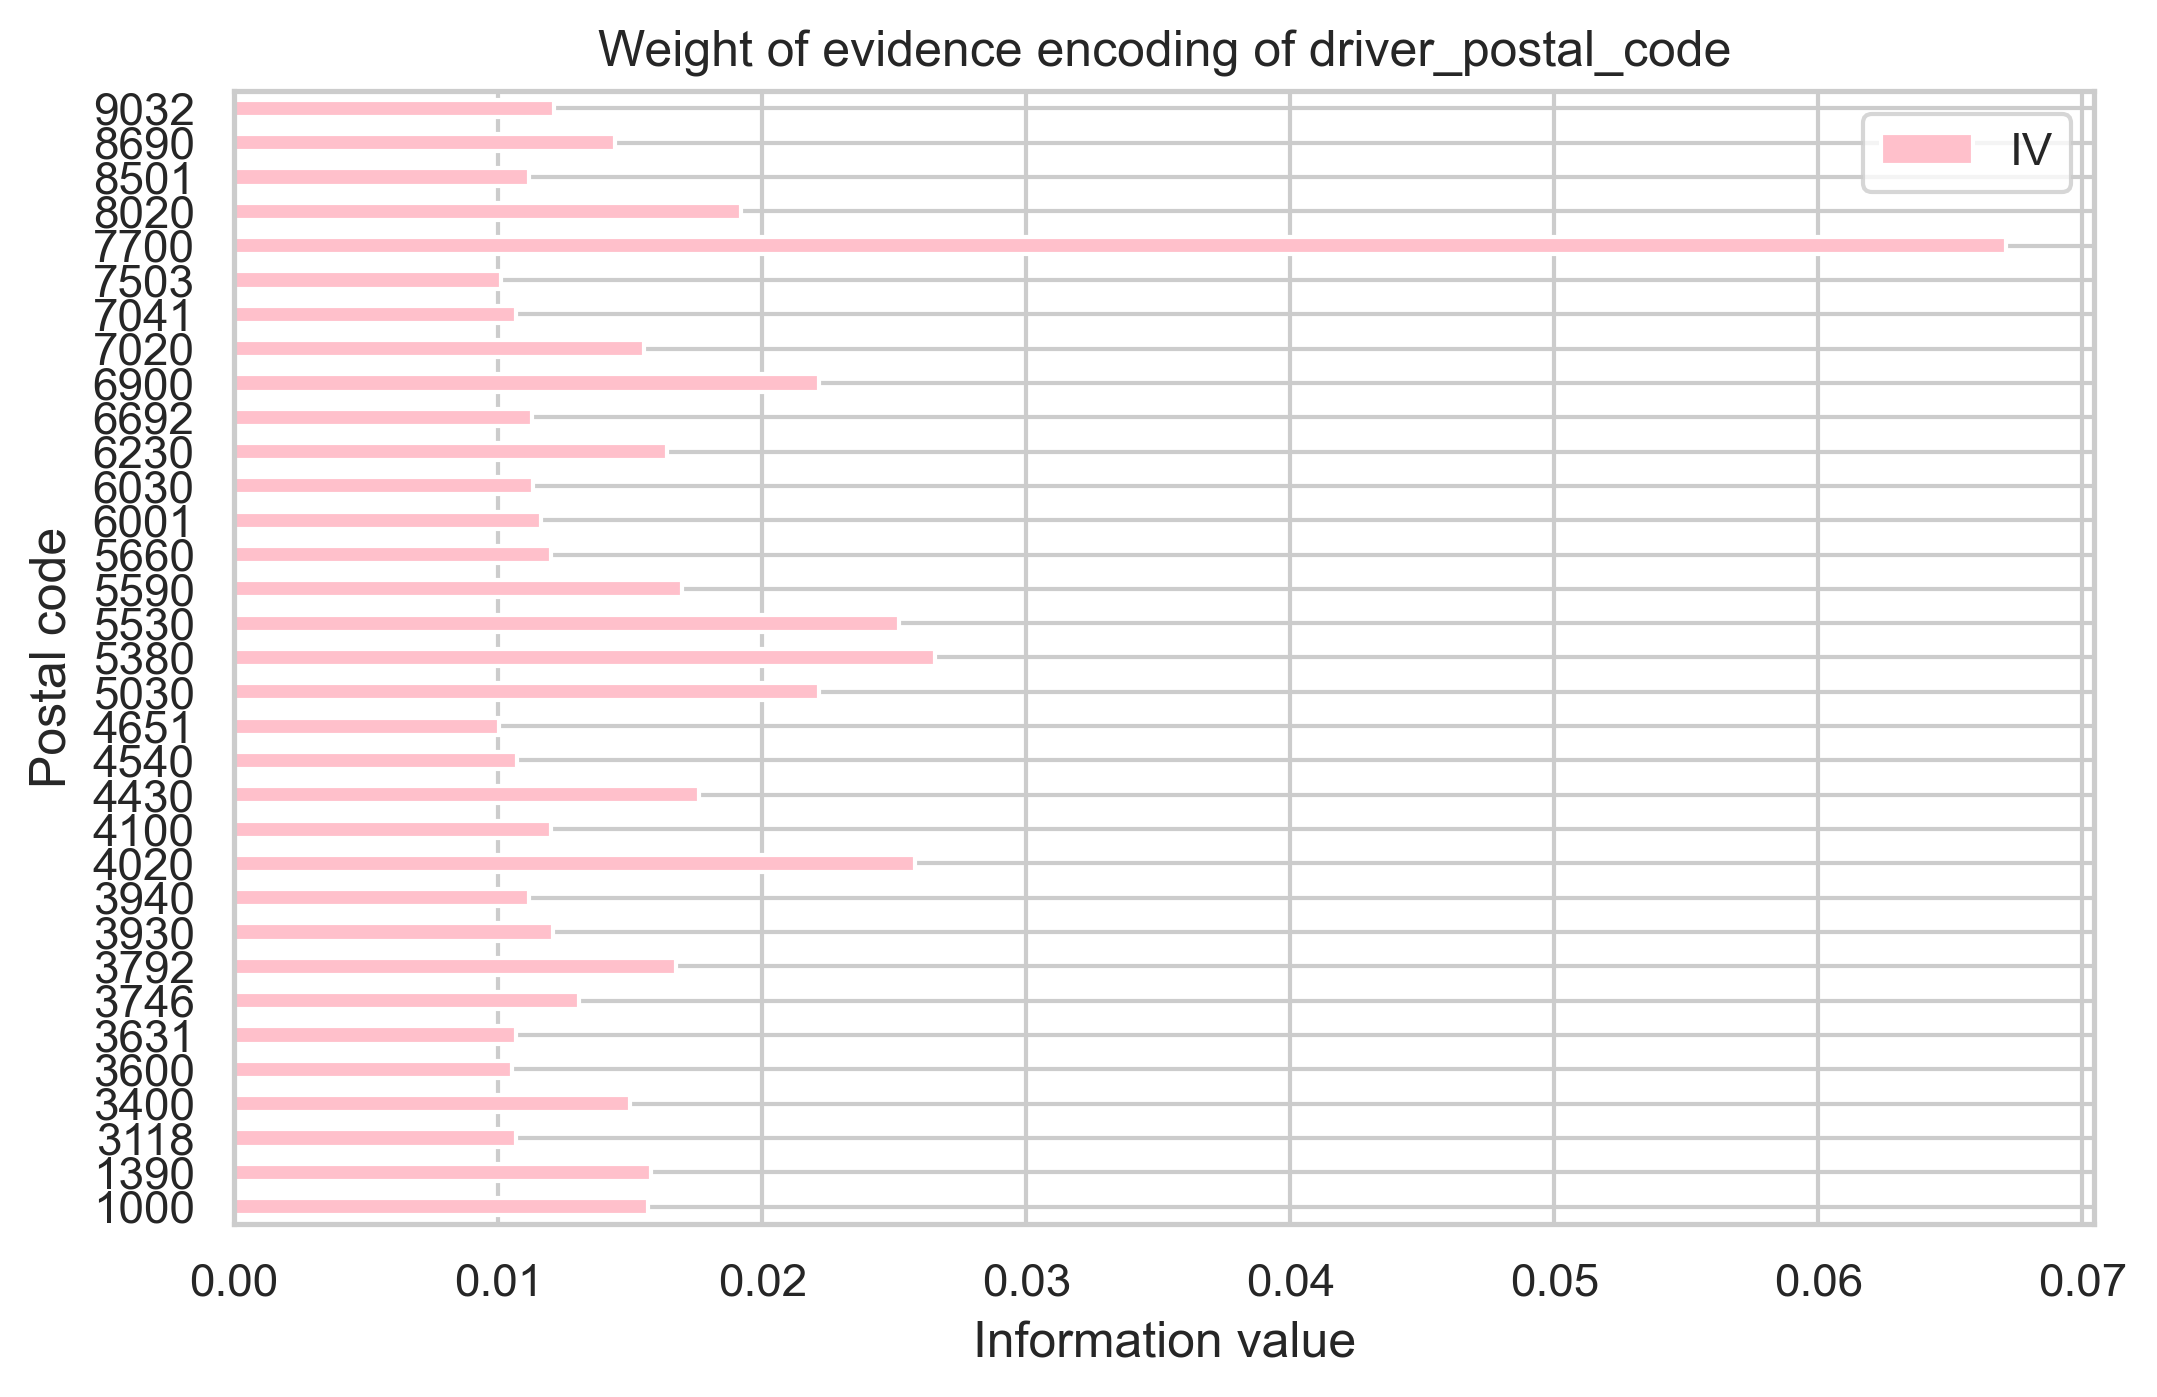
\includegraphics[width=1\linewidth]{info_val_driver_postal_code}
  \caption{\texttt{driver\_postal\_code}}
  \label{fig:sub2}
\end{subfigure}
\vspace{0.5cm}

\begin{subfigure}{.5\textwidth}
  \centering
  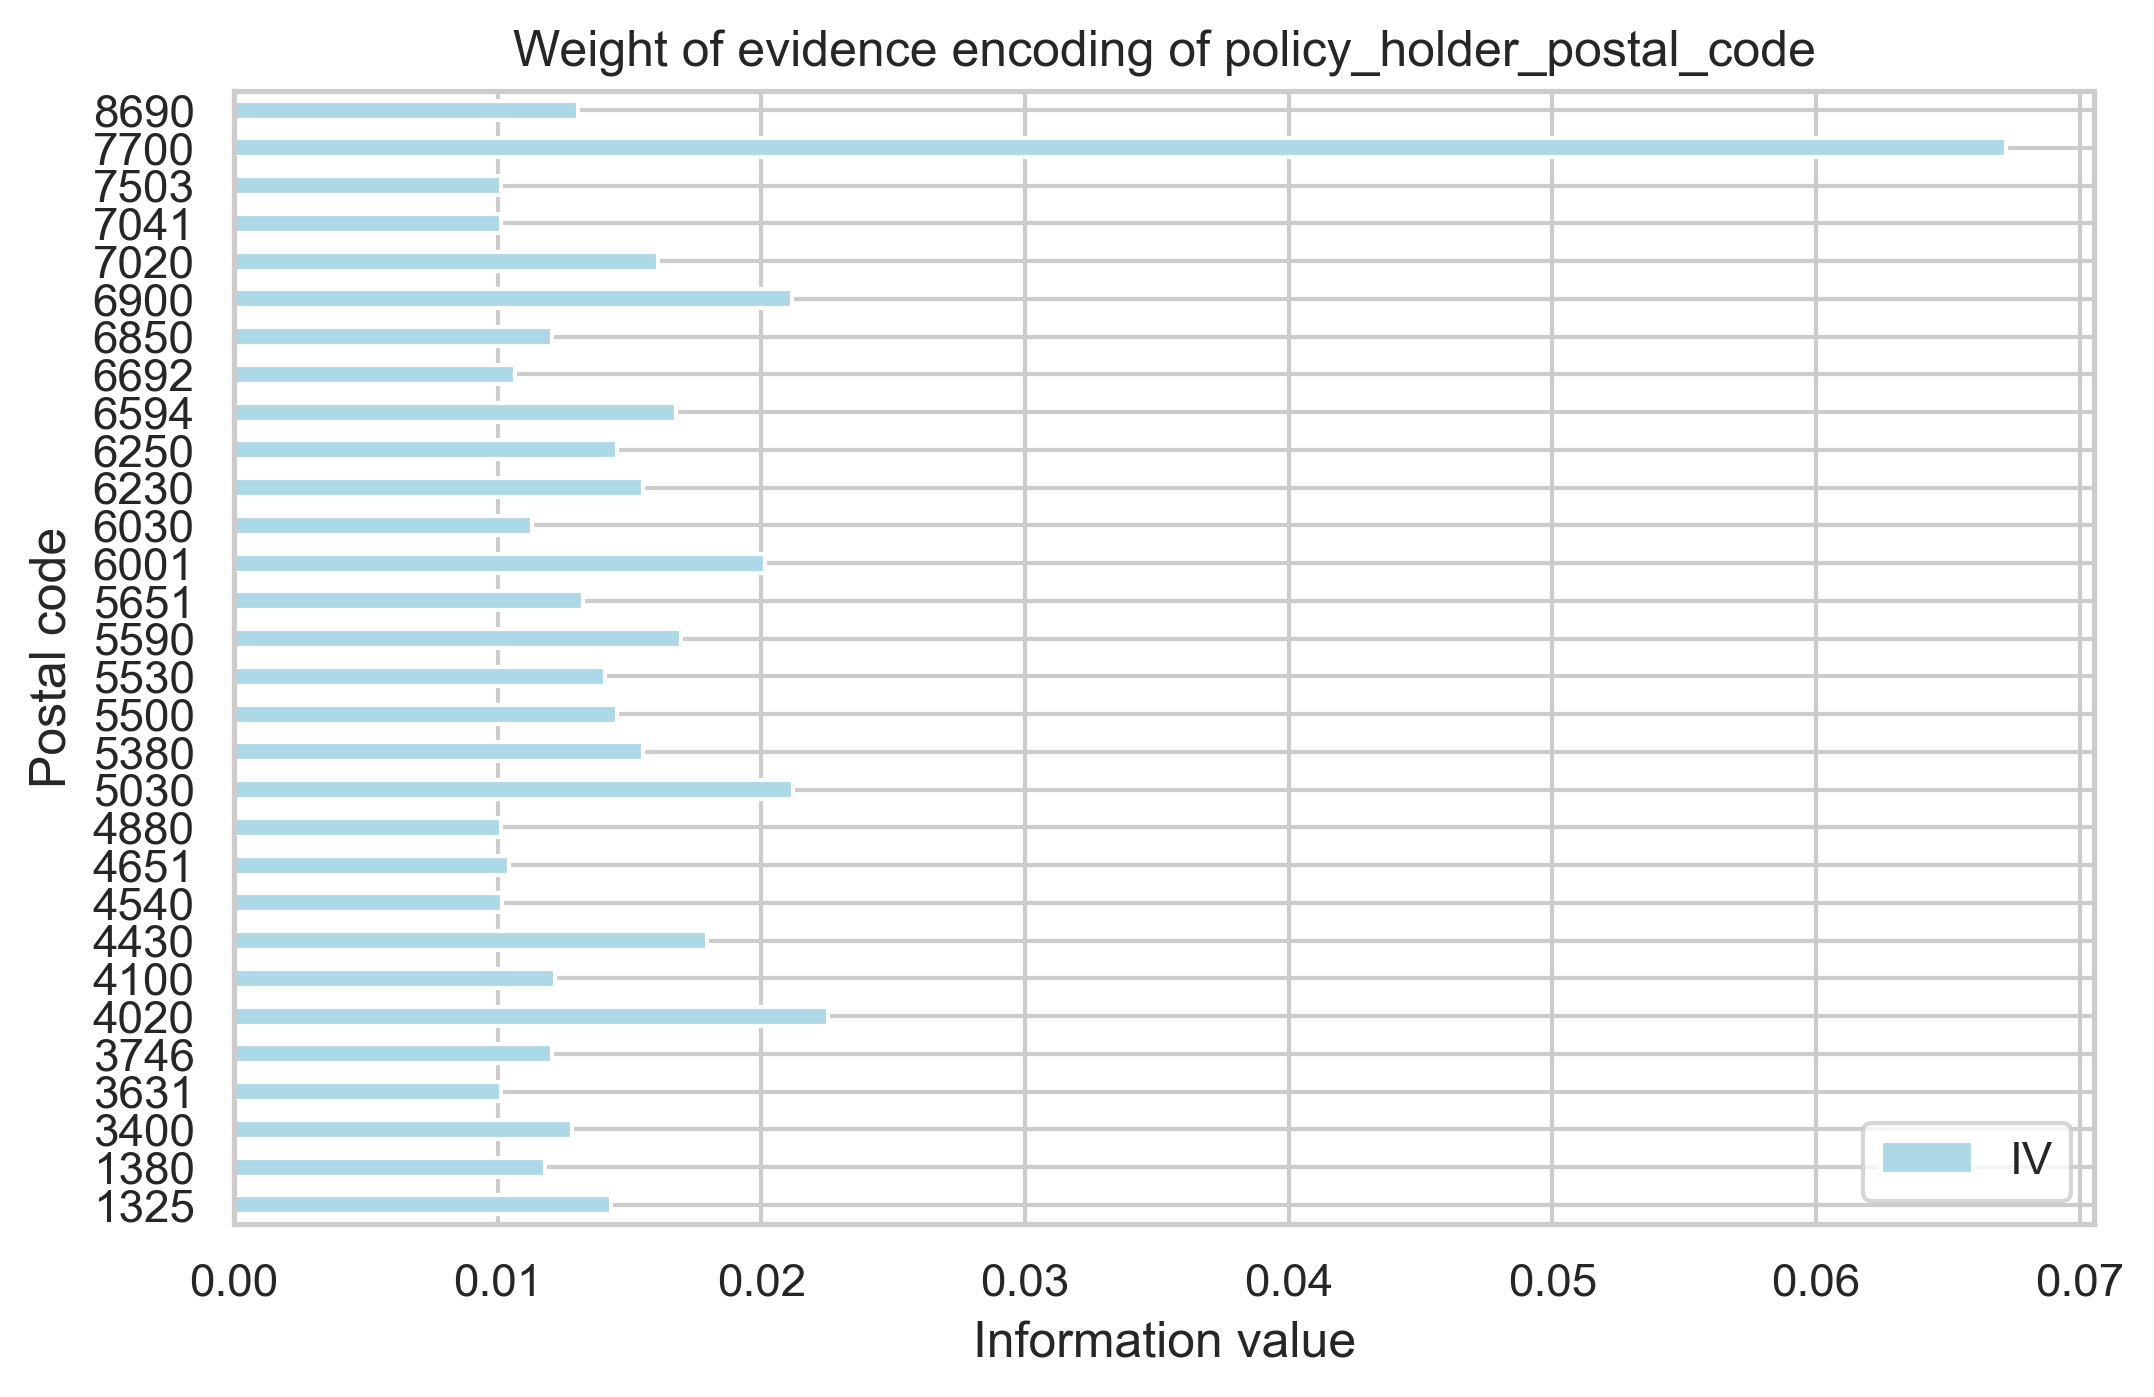
\includegraphics[width=1\linewidth]{info_val_policy_holder_postal_code}
  \caption{\texttt{policy\_holder\_postal\_code}}
  \label{fig:sub3}
\end{subfigure}%
\begin{subfigure}{.5\textwidth}
  \centering
  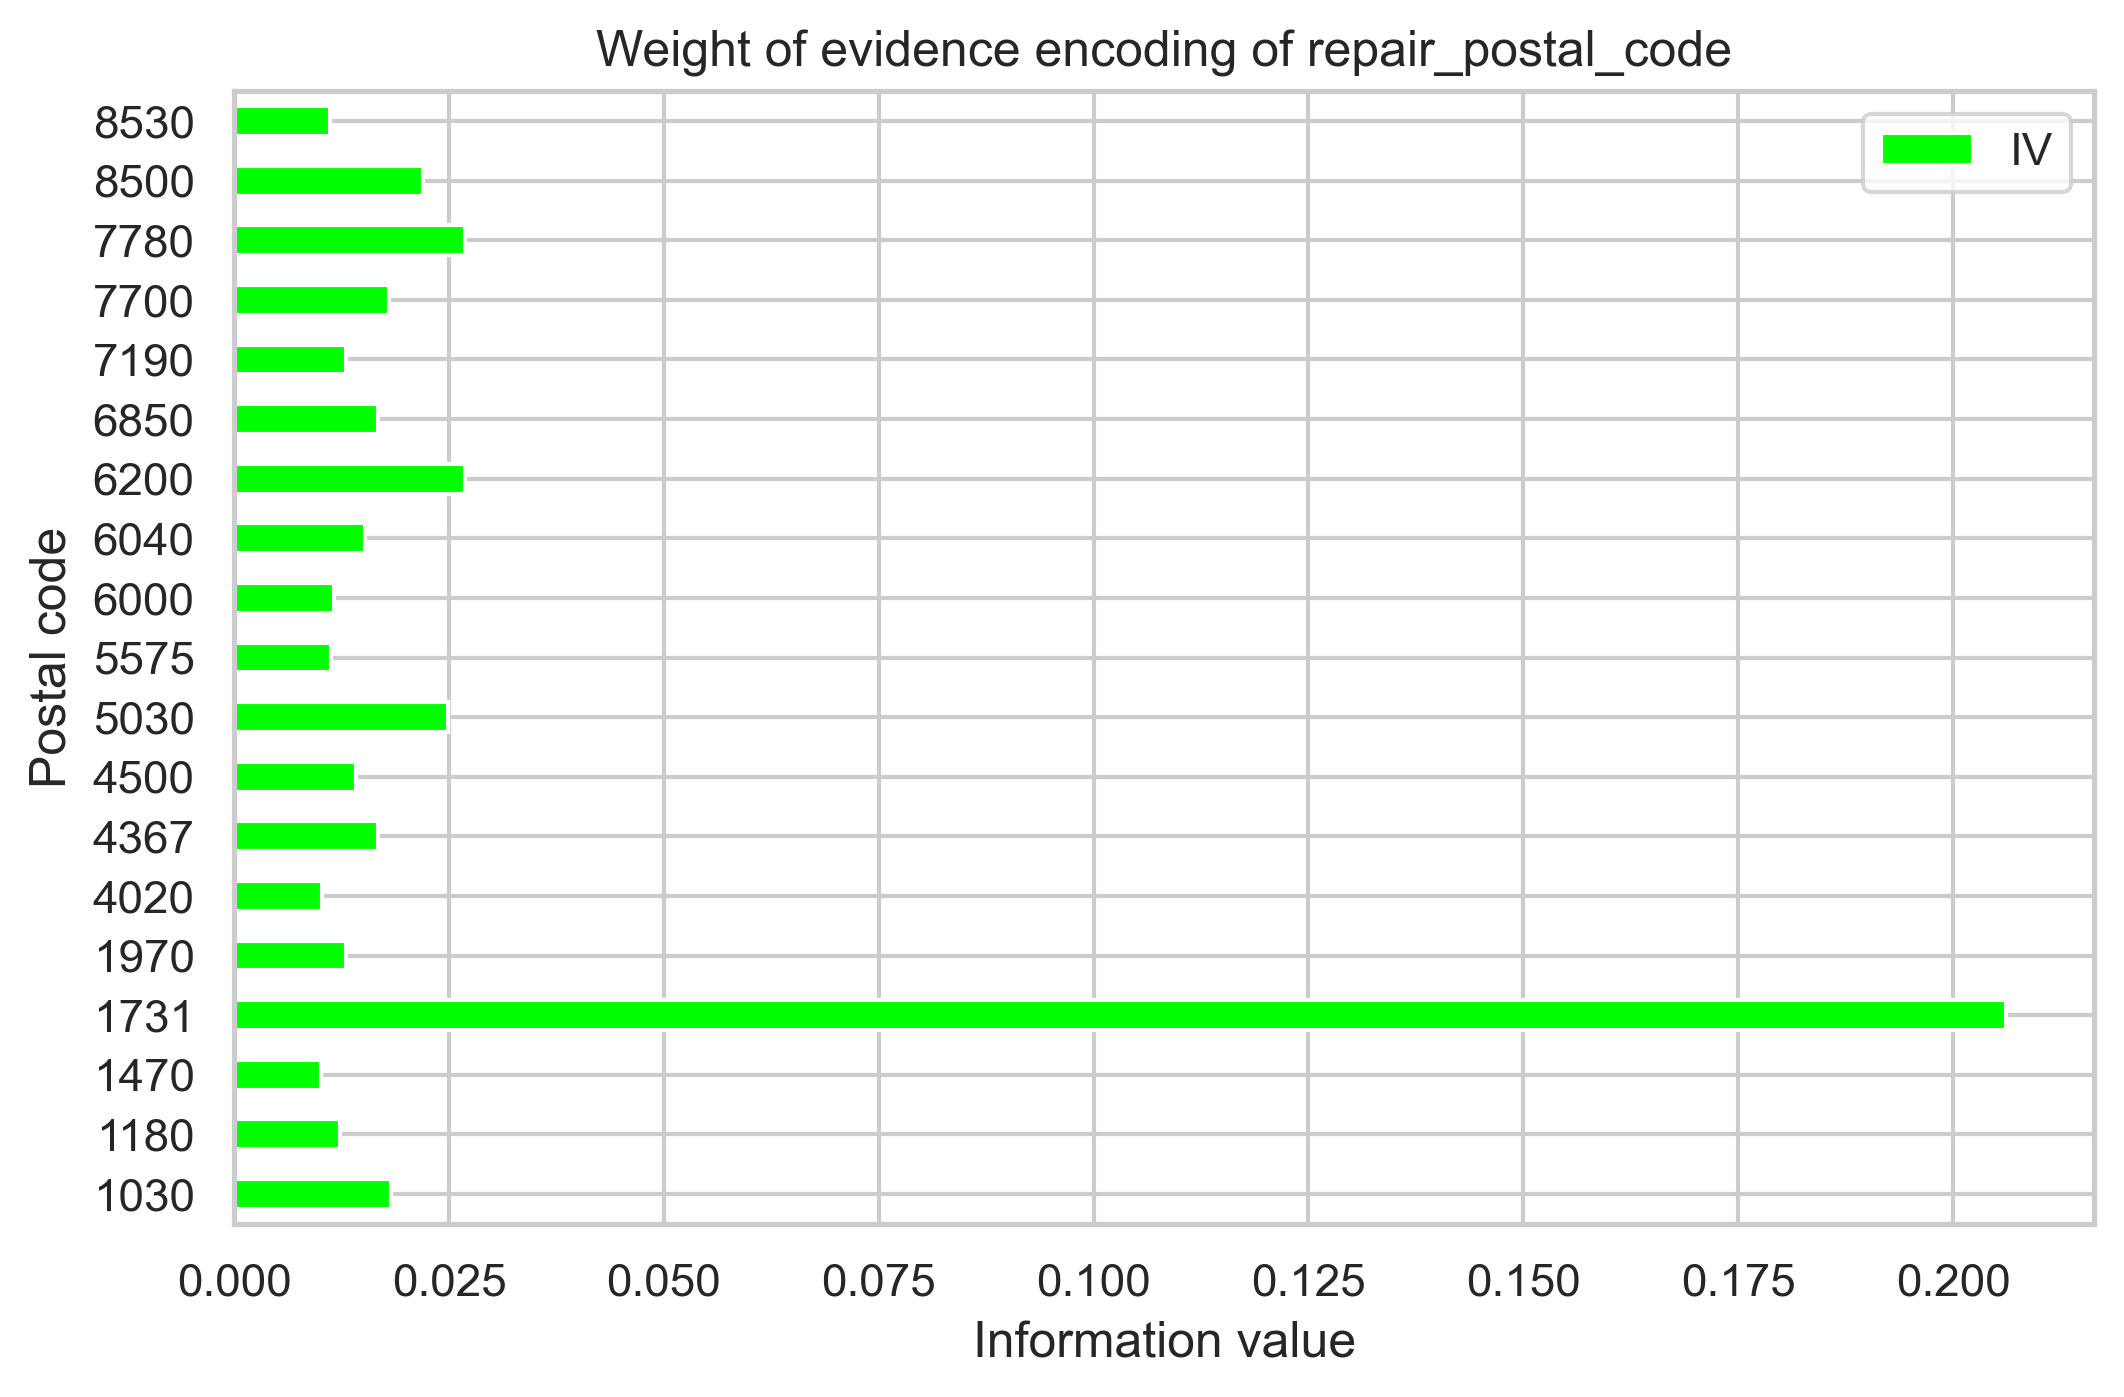
\includegraphics[width=1\linewidth]{info_val_repair_postal_code}
  \caption{\texttt{repair\_postal\_code}}
  \label{fig:sub4}
\end{subfigure}
\vspace{0.5cm}

\begin{subfigure}{.5\textwidth}
  \centering
  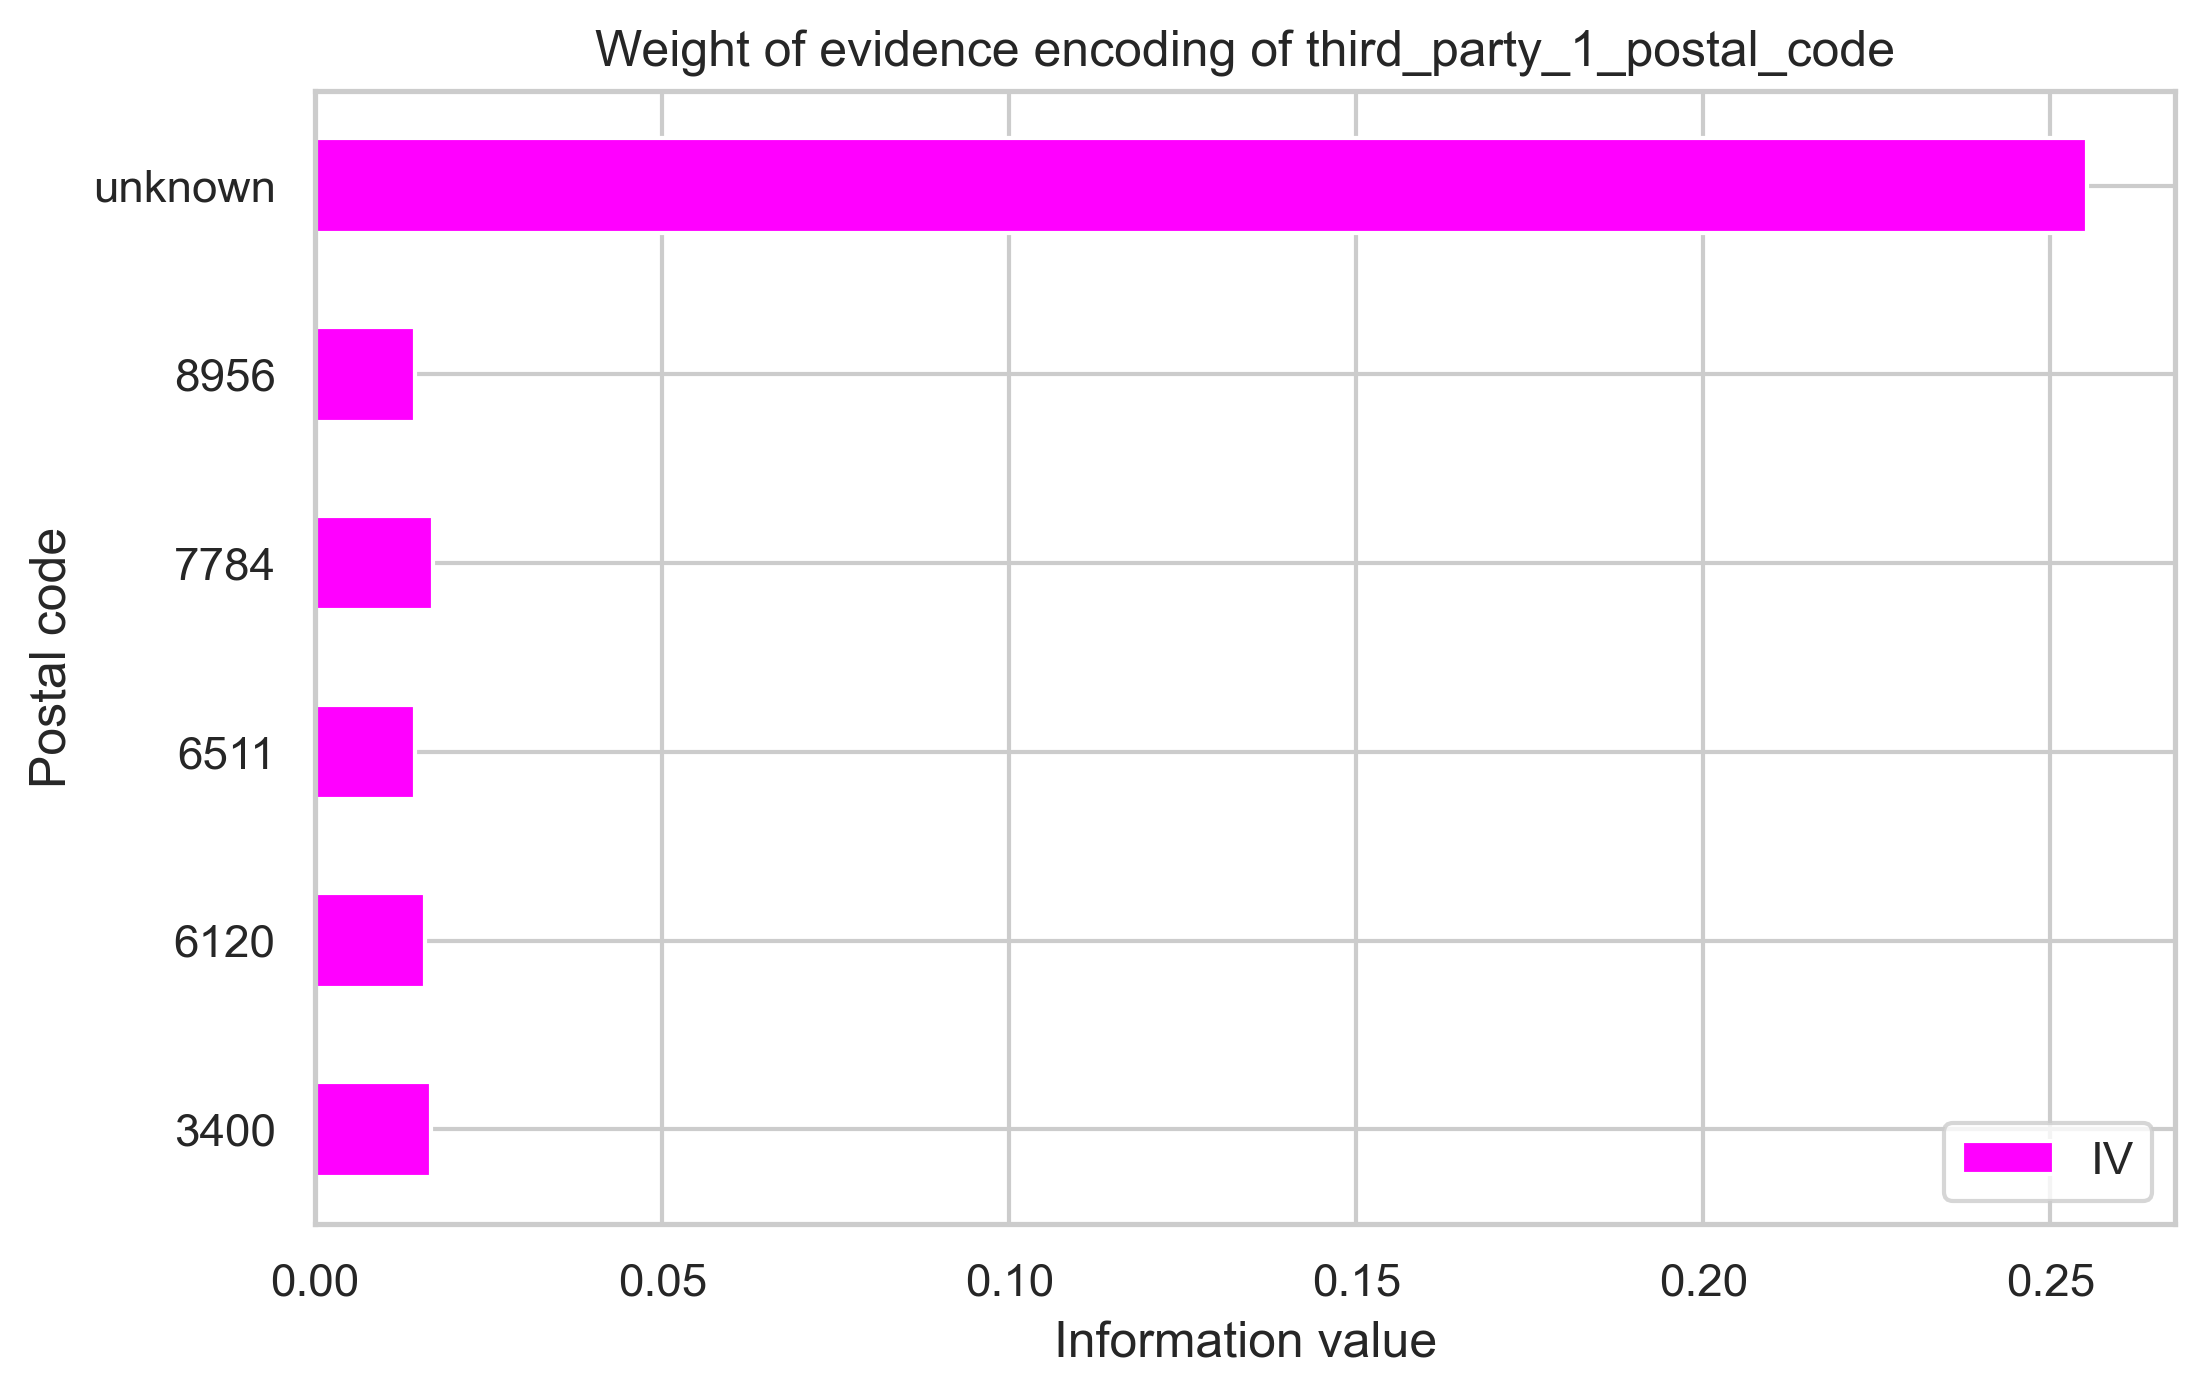
\includegraphics[width=1\linewidth]{info_val_third_party_1_postal_code}
  \caption{\texttt{third\_party\_1\_postal\_code}}
  \label{fig:sub5}
\end{subfigure}%
\begin{subfigure}{.5\textwidth}
  \centering
  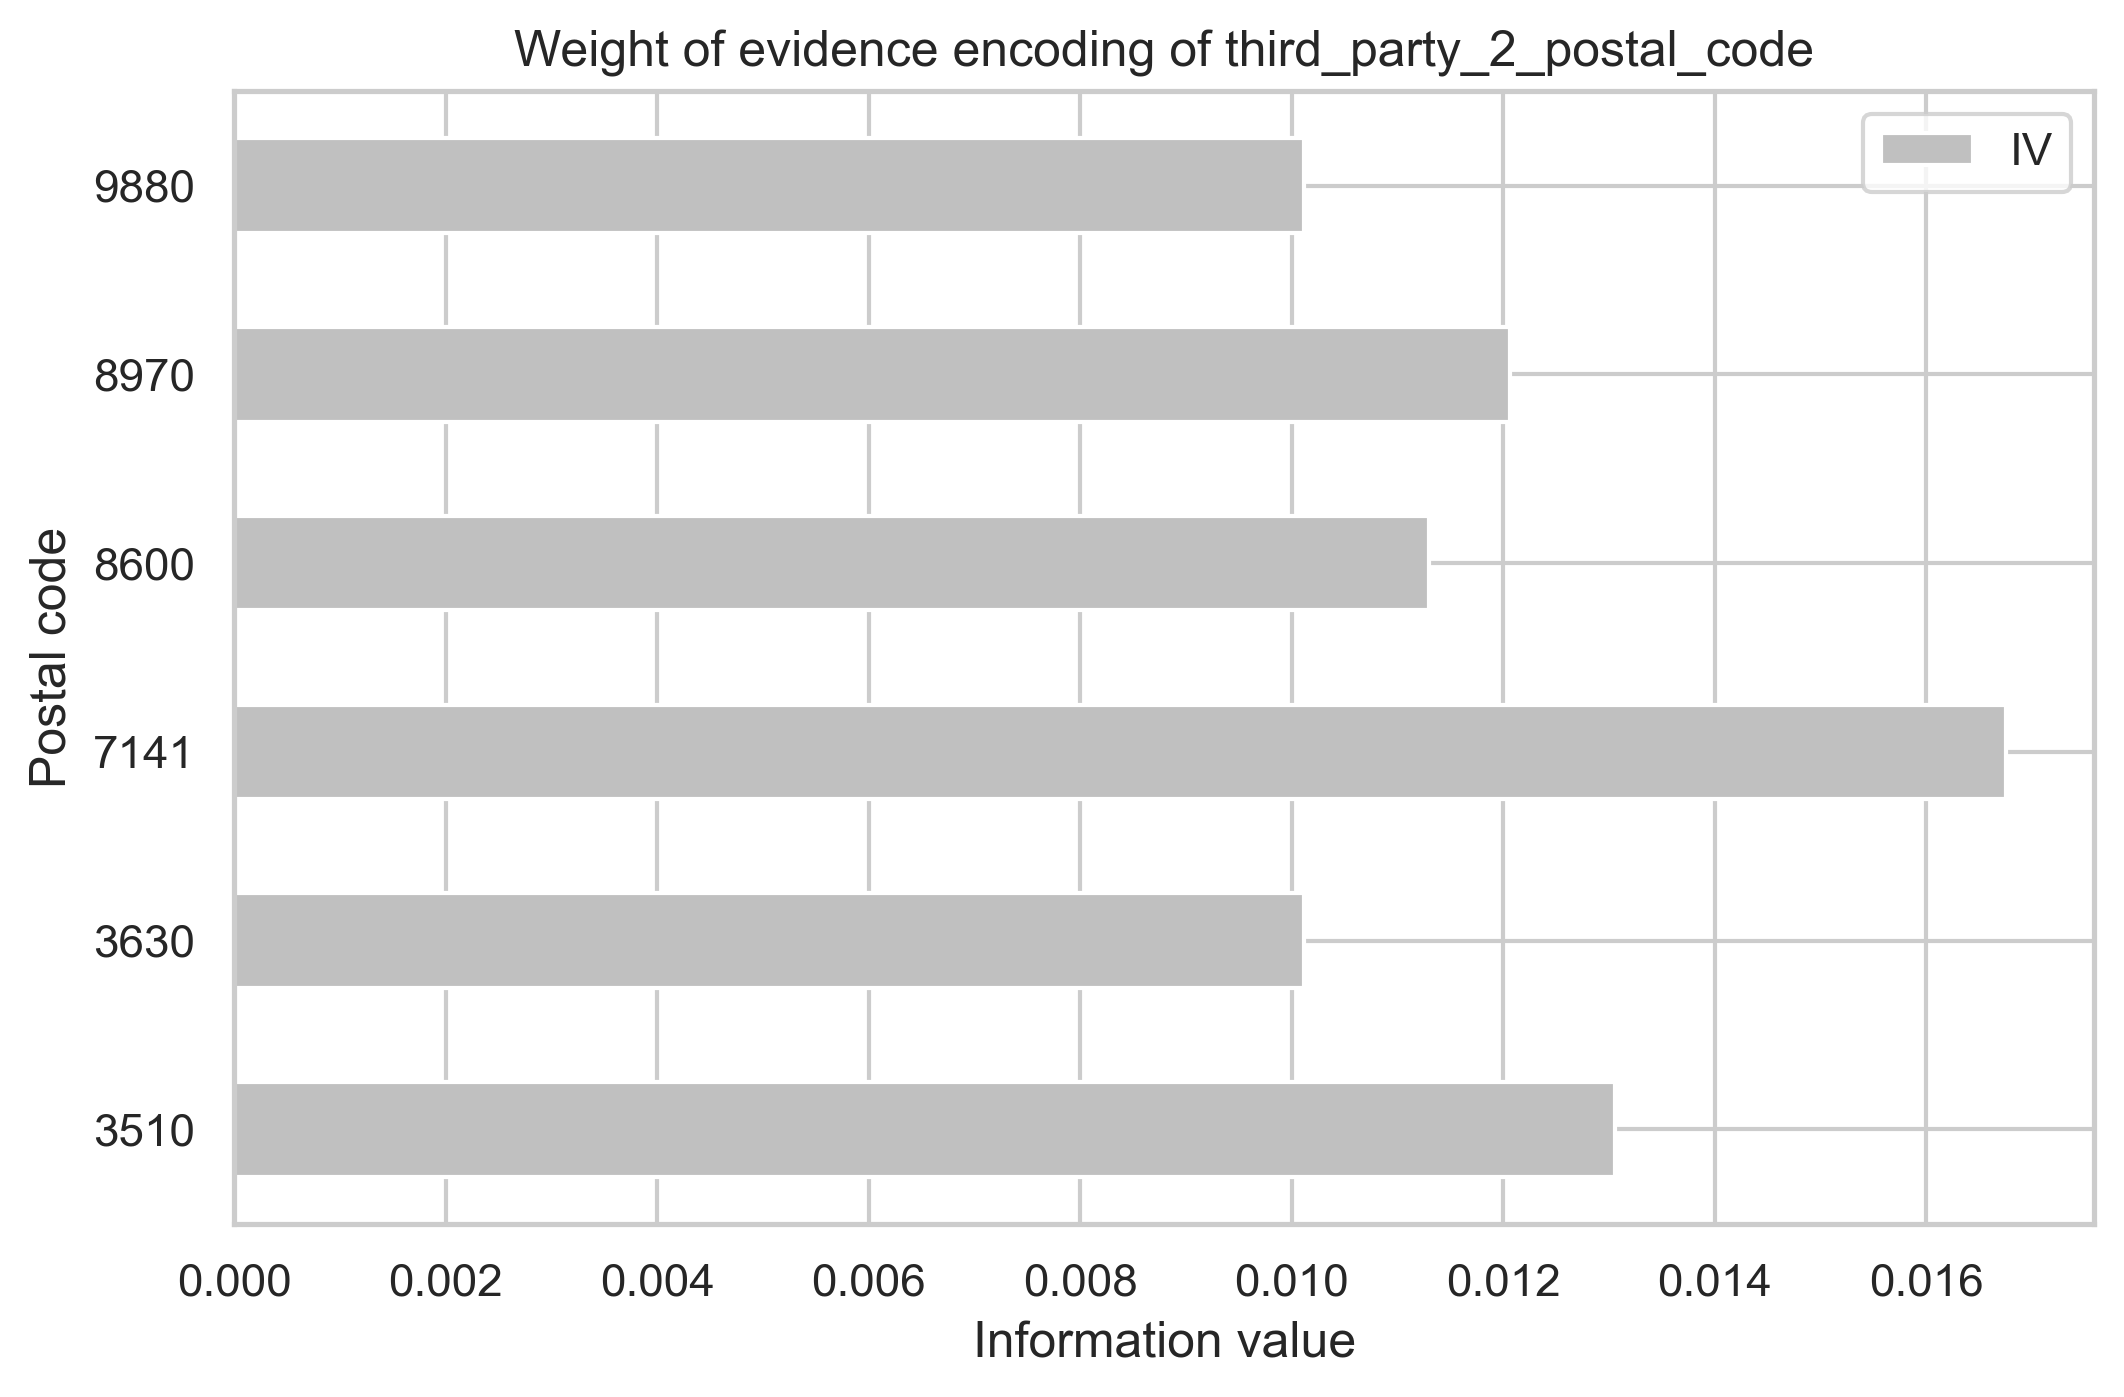
\includegraphics[width=1\linewidth]{info_val_third_party_2_postal_code}
  \caption{\texttt{third\_party\_2\_postal\_code}}
  \label{fig:sub6}
\end{subfigure}
\caption{Information values for postal code-related features}
\label{fig:iv_postal_code}
\end{figure}

\clearpage

\begin{figure}[h]
\centering
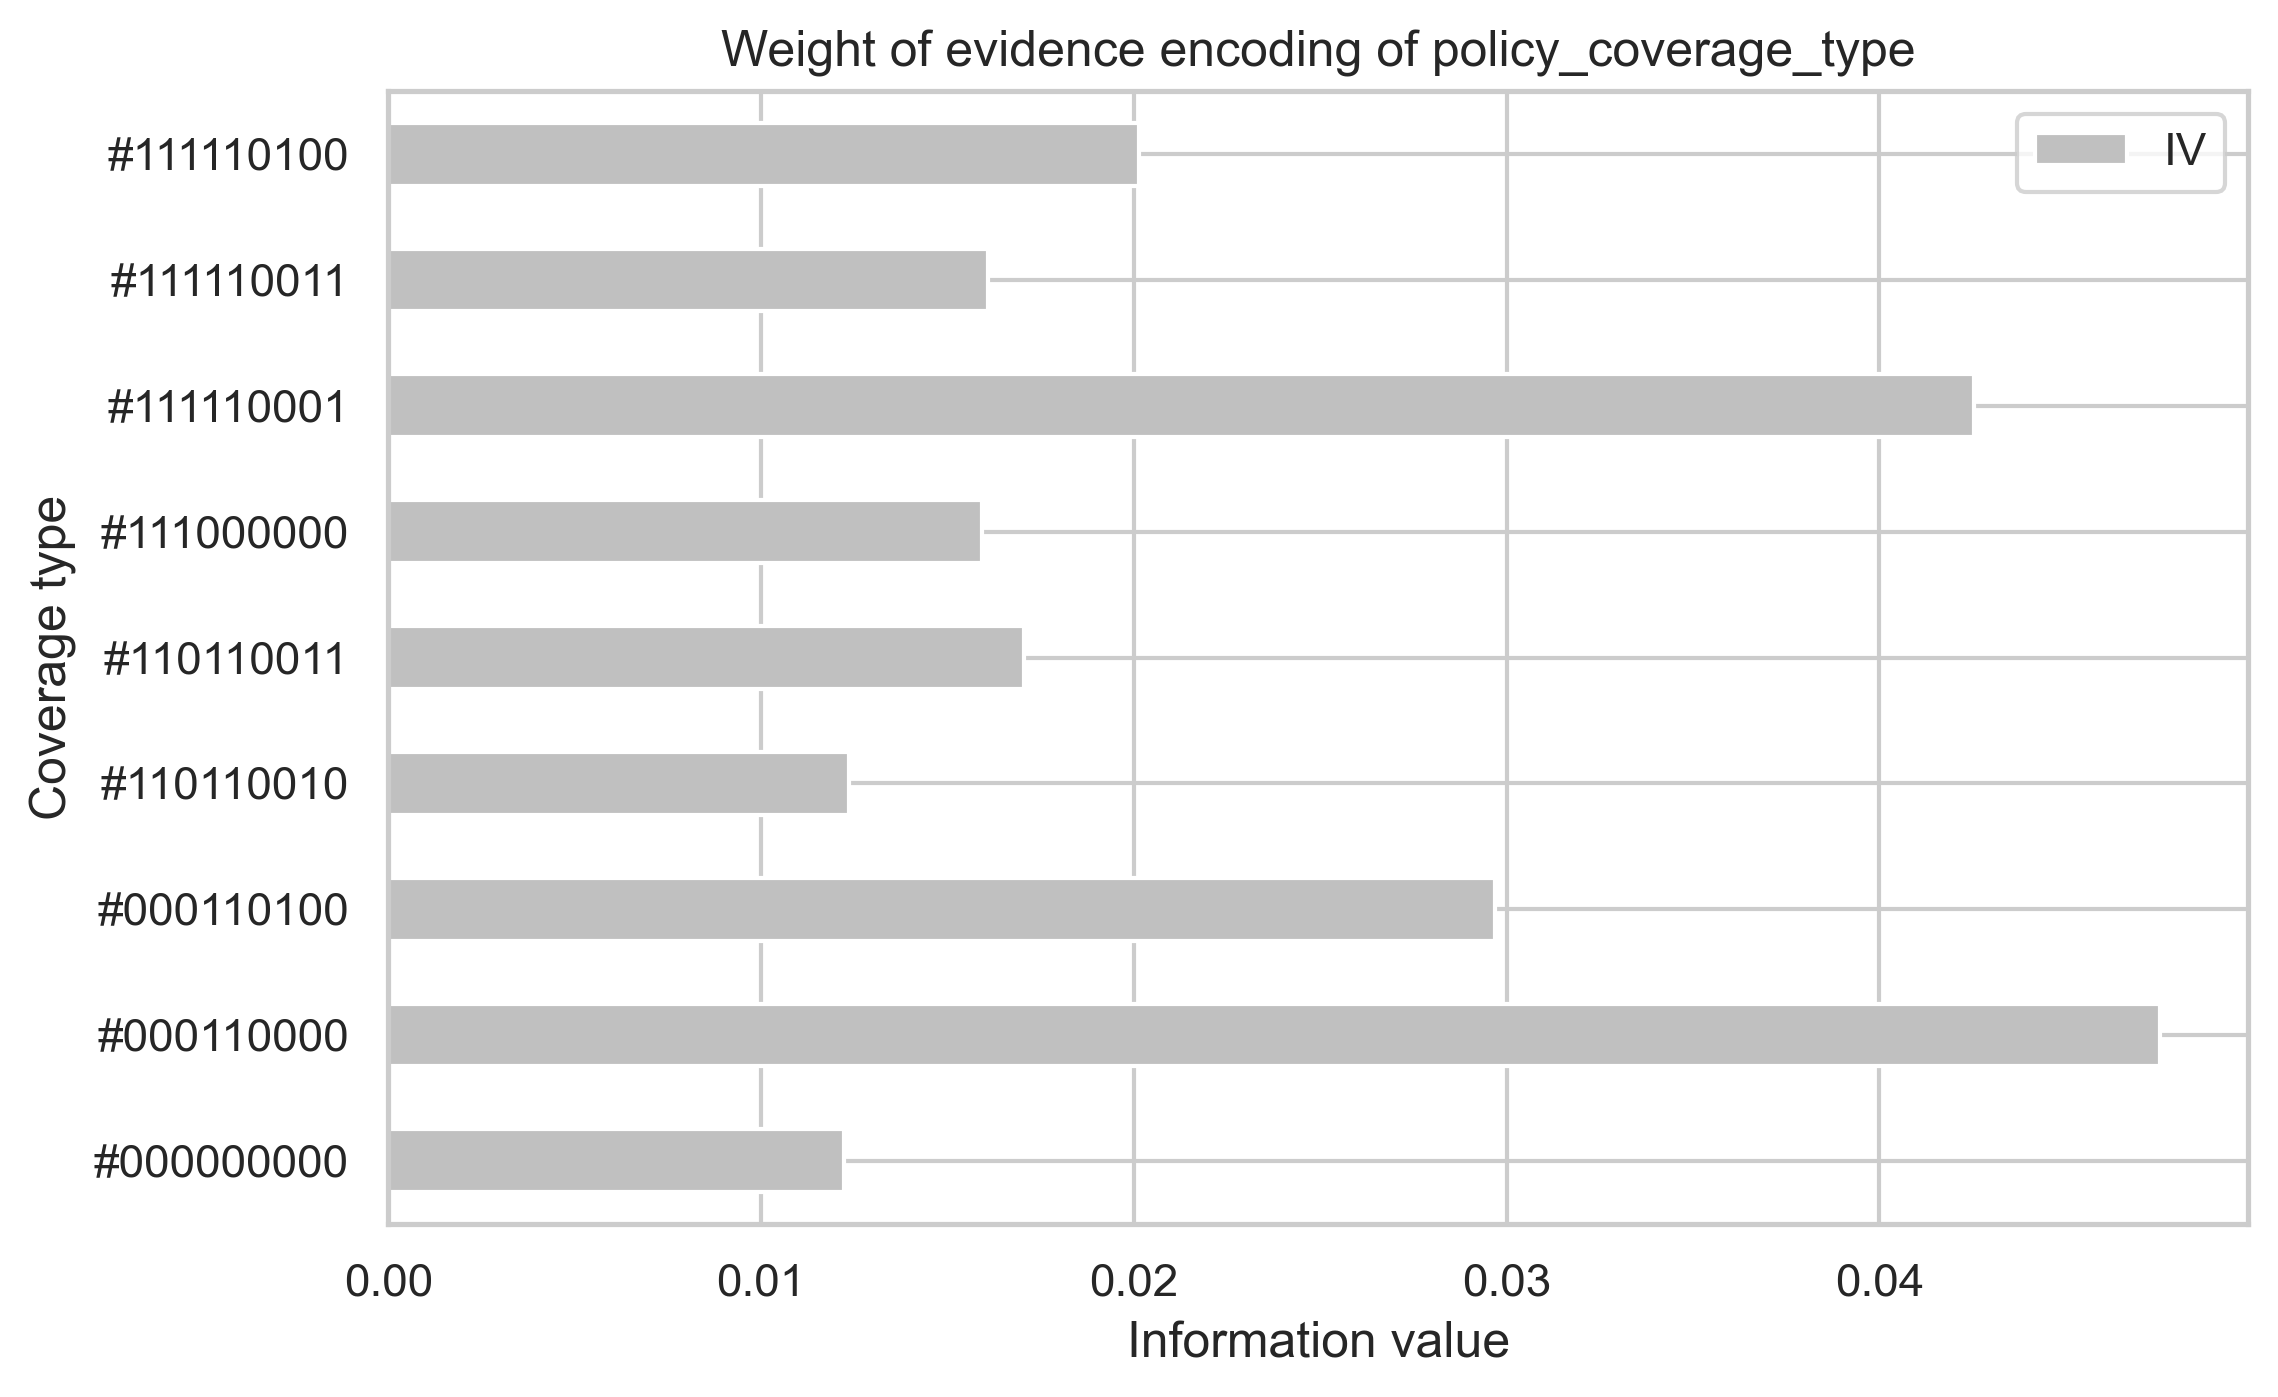
\includegraphics[width = 10cm, height = 7cm]{info_val_policy_coverage_type}
\caption{Information values for policy coverage types}
\end{figure}


\subsubsection*{Multivariate analysis}
\addcontentsline{toc}{subsubsection}{Multivariate analysis}

High correlation among features may indicate the existence of some redundant features. Therefore, a correlation plot is presented in figure 14, and we observe that the correlation among \texttt{policy\_coverage\_1000} and \texttt{claim\_vehicle\_cyl} and \texttt{claim\_vehicle\_power} are strong. And the correlation between \texttt{driver\_age} and \texttt{policy\_holder\_age} are also strong. There may be some common factors behind correlated features. Although the correlations are strong. Instead of dropping them, we can discretize the features to reduce the correlation and preserve information as they are not 100\% correlated. As discussed in previous section, age-related features are discretized. Moreover, we will discretize \texttt{policy\_coverage\_1000} because it has more than 50\% of missing values and a strong correlation.

\begin{figure}[h]
\centering
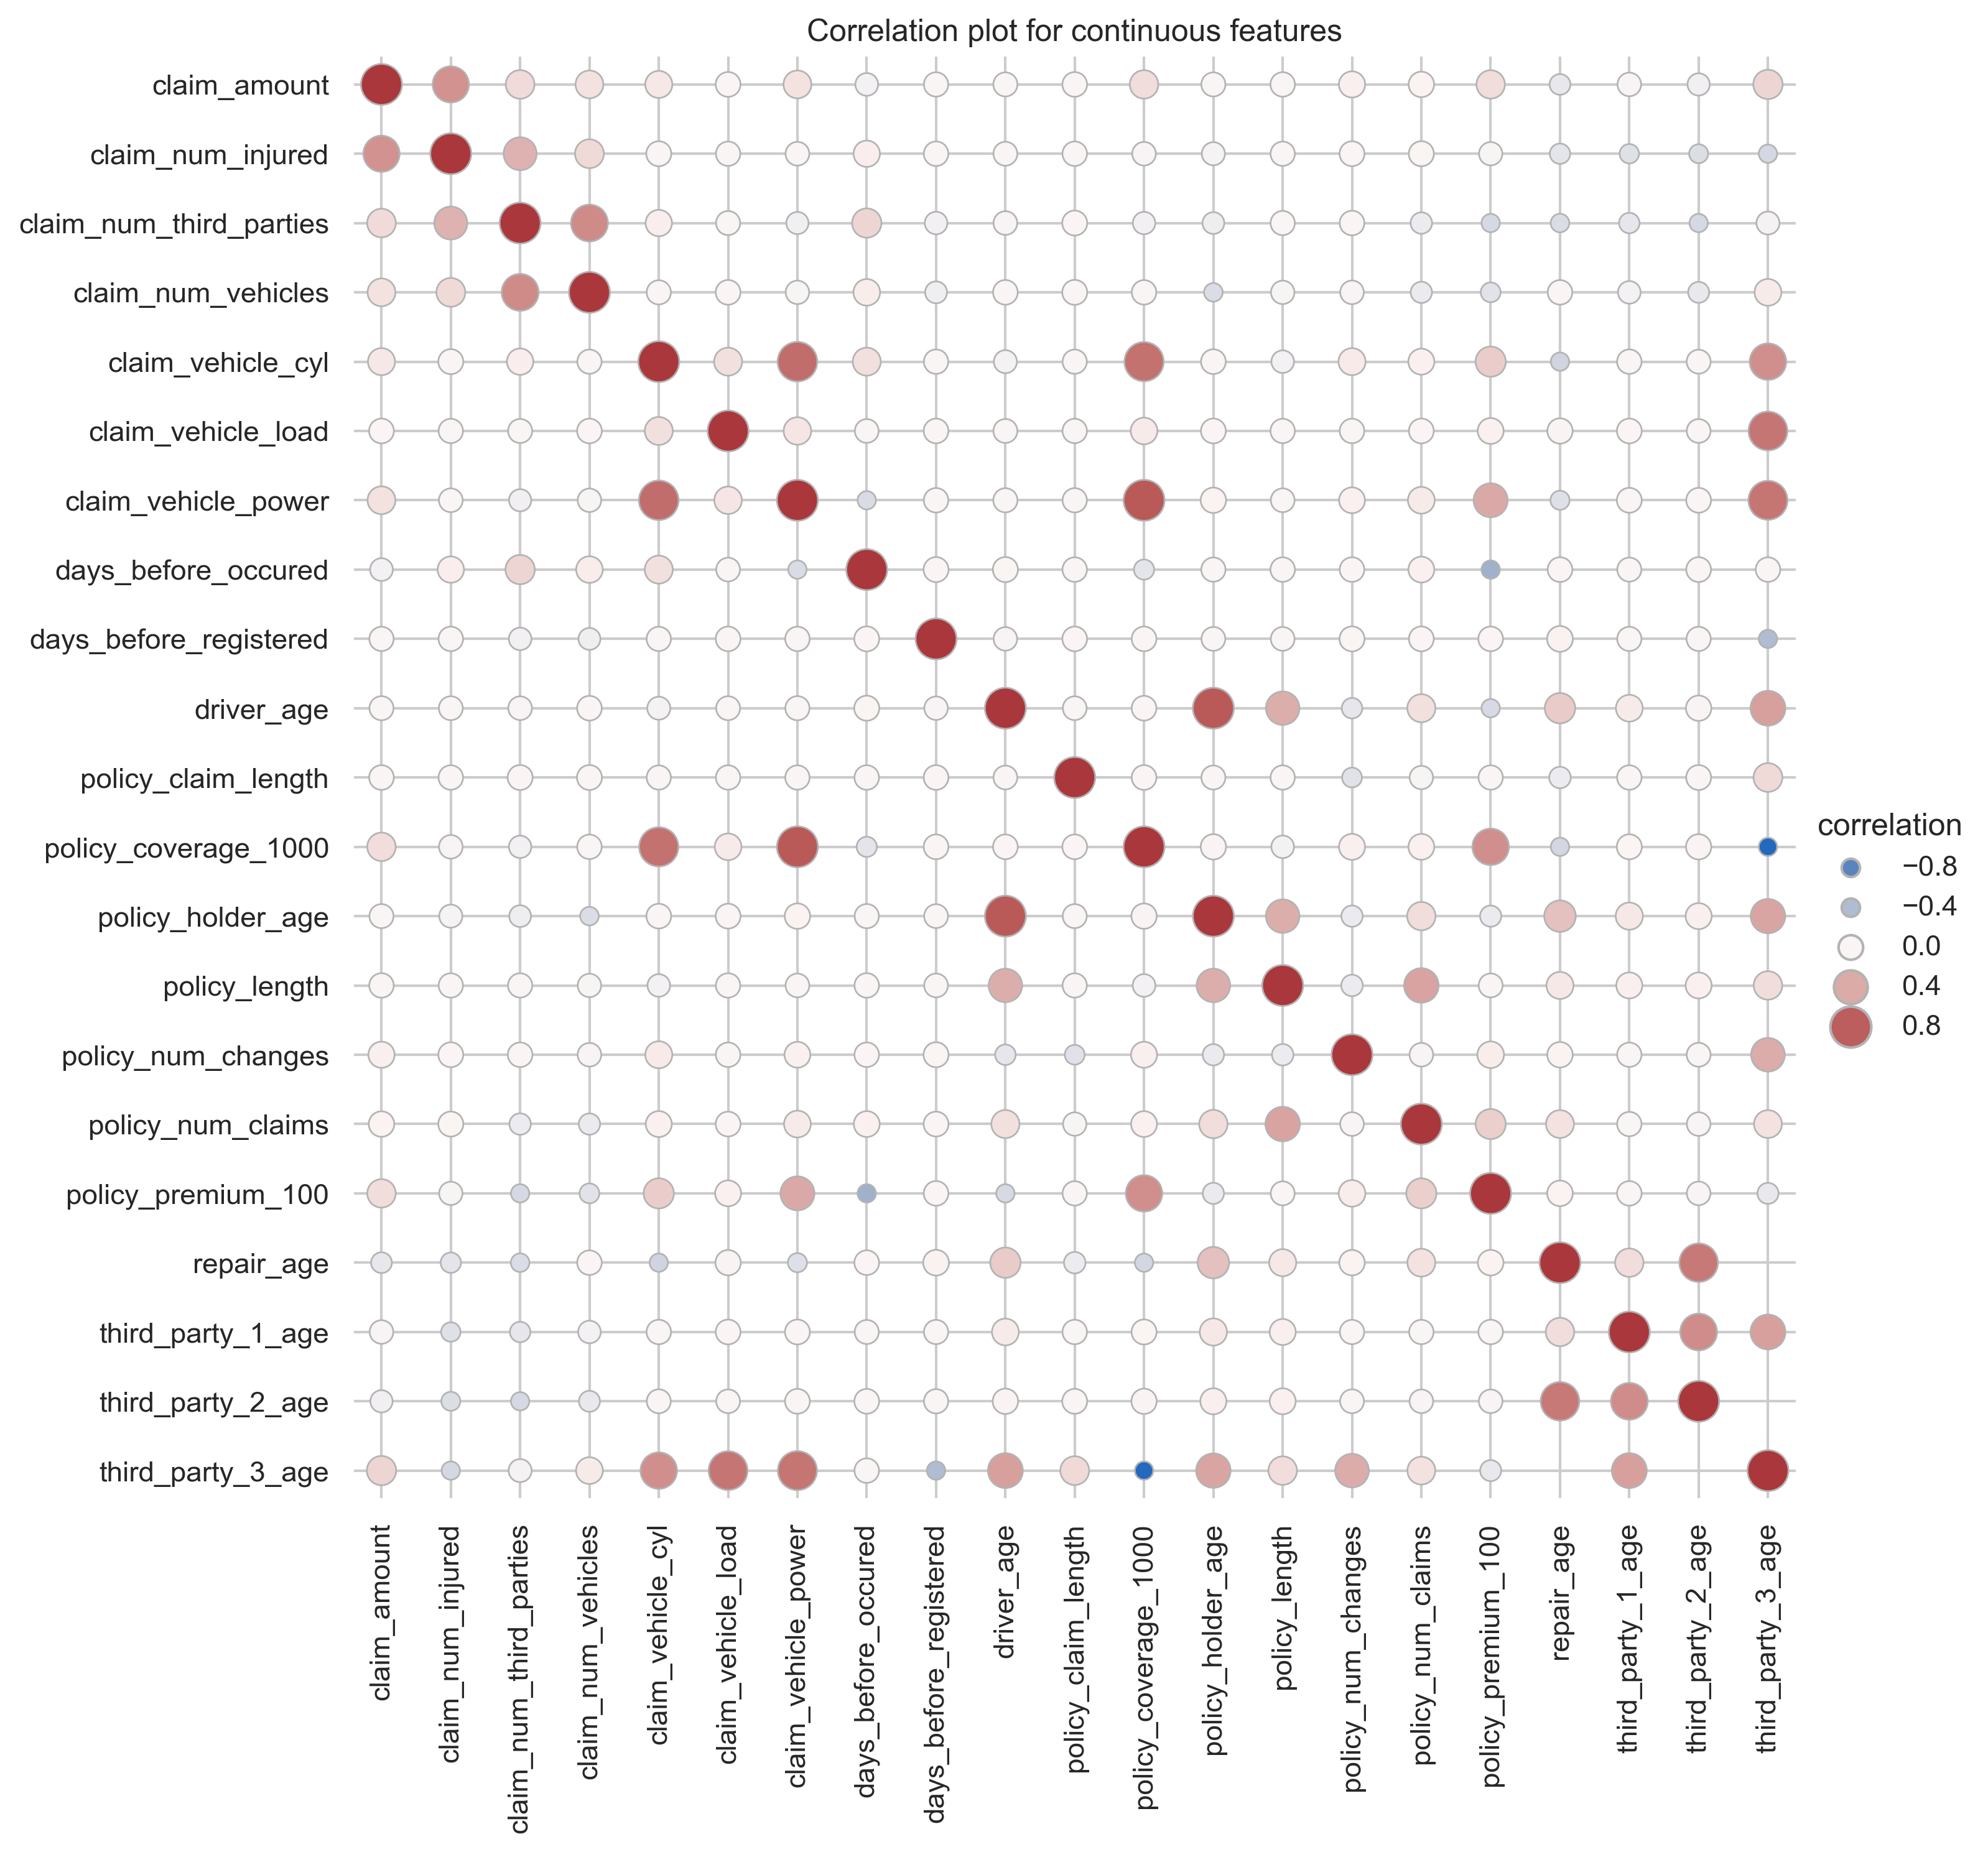
\includegraphics[width = 14cm, height = 12cm]{corr_plot}
\caption{Correlation plot for continuous features}
\end{figure}



\subsubsection*{Unsupervised learning}
\addcontentsline{toc}{subsubsection}{Unsupervised learning}

\subsection*{Model building}
\addcontentsline{toc}{subsection}{Model building}

\subsubsection*{Algorithms}
\addcontentsline{toc}{subsubsection}{Algorithms}

\subsubsection*{Probability Calibration}
\addcontentsline{toc}{subsubsection}{Probability Calibration}

\subsubsection*{Metrics and Grid Search}
\addcontentsline{toc}{subsubsection}{Metrics and Grid Search}

\subsubsection*{Data pipeline}
\addcontentsline{toc}{subsubsection}{Data pipeline}

\subsubsection*{Model Comparison}
\addcontentsline{toc}{subsubsection}{Model Comparison}


\subsection*{Interpretation}
\addcontentsline{toc}{subsection}{Interpretation}

\subsection*{Reflection}
\addcontentsline{toc}{subsection}{Reflection}

\clearpage
\section*{Assignment 2}
\addcontentsline{toc}{section}{Assignment 2}

\clearpage
\section*{Assignment 3}
\addcontentsline{toc}{section}{Assignment 3}

\clearpage
\section*{Assignment 4}
\addcontentsline{toc}{section}{Assignment 4}
\end{document}